%--------------------------------------------%
% Template Beamer para Apresentações da UFRN %
% by alcemygvseverino@gmail.com              %
% Baseado em MIT Beamer Template			 %
% versao 1.1								 %
% Atualizado em 14/05/2016					 %
%--------------------------------------------%
\documentclass[handout,t]{beamer}
% Para alterar a linguagem do documento
\usepackage[portuges]{babel}
% Para aceitar caracteres especias deretamente do teclado
\usepackage[utf8]{inputenc}
% Para seguir as normas da ABNT de citacao e referencias
\usepackage[alf]{abntex2cite}
% Para incluir figuras
\usepackage{graphicx}
% Para melhor ajuste da posisao das figuras
\usepackage{float}
% Para ajustar as dimensoes do layout da pagina
\usepackage{geometry}
% Para formatar estrutura e informacoes de formulas matematicas
\usepackage{amsmath}
% Para incluir simbolos especiais em formulas matematicas
\usepackage{amssymb}
% Para incluir links nas referencias
\usepackage{url}
% Para incluir paginas de documentos .pdf externos
\usepackage{pgfpages}
% Para ajustar o estilo dos contadores
\usepackage{enumerate}
% Para modificar a cor do texto
\usepackage{color}
% Para incluir condicoes
\usepackage{ifthen}
% Para colocar legendas em algo que nao e float
\usepackage{capt-of}
\usepackage{subcaption}
\usepackage{bm}

% Para definir o tema do slide
\usetheme{Berlin}
% Para difinir cores e background
\usecolortheme{ufrn}
% Para numerar as figuras
\setbeamertemplate{caption}[numbered]

% Título
\title[Trabalho de Conclusão de Curso]{
	Controle Embarcado para Robôs com Acionamento Diferencial e \emph{Encoders} de Baixa Resolução.}
% Data
\date{
% 	\today
    14 de dezembro de 2020
}
% Autores
\author[Luís Gabriel]{
	Autor:Luís Gabriel Pereira Condados \inst{1}\\
	\vspace{0.25cm}
	Orientador:Adelardo Adelino Dantas de Medeiros \inst{2}}
% Instituto
\institute[INSTITUTO]{
	\inst{1}%
	\url{gabriellgpc@hotmail.com}\\
	\vspace{0.25cm}
	\inst{1,2}%
	Departamento de Engenharia de Computação e Automação (DCA)\\
	Universidade Federal do Rio Grande do Norte}
% Logo do canto inferior direito
\pgfdeclareimage[height=0.7cm]{logo_UFRN}{figuras/logo_UFRN}
\logo{
	\vspace*{-0.25cm}
	\pgfuseimage{logo_UFRN}
	\hspace*{-0.05cm}}


\begin{document}
% Sumário
\frame{\titlepage}
\section[]{}
\begin{frame}{Sumário}
	\tableofcontents
\end{frame}

% Introducao
\section{Introdução}

% Uma forma muito comum de acionamento de motores de corrente continua (CC) é por meio da modulação por largura de pulso, ou do inglês Pulse Width Modulation (PWM), que consiste basicamente em manipular a tensão média de alimentação do motor por meio de sinais digitais. É comum em certas aplicações o uso do sinal \emph{PWM} para manipular a velocidade do motor, ou seja, um controle de malha aberta, esse tipo de sistema apenas regula o quão rápido o motor irá girar. Porém na maioria das aplicações o controle em malha aberta não é suficiente, como por exemplo, não há garantias que se aplicadas tensões iguais (\emph{PWM}) em ambos os motores de um robô com acionamento diferencial (robôs com duas rodas tracionadas e independentes) o movimento será estritamente linear \cite{simple_speed_feedback}, isso é devido às diferenças entre os dois conjuntos de motores/rodas que fazem com que esses não girem a uma mesma velocidade, mesmo sobre uma mesma tensão.\\

% Existem diversos desafios no projeto de robôs pequenos, além da questão mecânica, o tamanho reduzido também restringe a possibilidade de se usar \emph{Hardwares} com mais capacidade computacional, além dos tipos e a quantidade de sensores que podem ser usados. Robôs como os da equipe Poti de Futebol de robôs (do Departamento de Computação e Automação (DCA) da UFRN), que são voltados para a participação na \emph{Latin American Robotic Competition} (LARC) na categoria \emph{IEEE Very Small Size Soccer} (VSSS), têm dificuldades para conseguirem comportar um \emph{Hardware} capaz de executar um controle digital de velocidade para ambos os motores, além de possuírem sensores com uma baixa acurácia, dificultando assim o bom desempenho do sistema de controle.\\

% O objetivo geral deste trabalho é projetar um sistema que realize o controle de velocidade dos motores de um robô com acionamento diferencial e que utiliza um estimador de velocidade sobre medições feitas com \emph{Encoders} de baixa resolução. Para a validação do trabalho foi feito a implementação do sistema proposto, testado em robôs reais e feito análises da eficiência dos controladores com relação à diminuição das assimetrias dos conjuntos motor-roda, bem como a qualidade da filtragem/estimativa da velocidade.

\begin{frame}{Motivação}
    \begin{figure}[H]
        \begin{subfigure}{.5\textwidth}
        \centering
        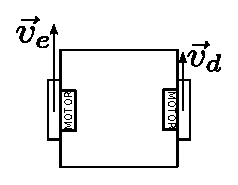
\includegraphics[width=0.5\textwidth]{figuras/ilustracoes/ilustracao_robo_diferentes_velocidades.eps}
        \end{subfigure}
        \begin{subfigure}{.5\textwidth}
        \centering
        
\includegraphics[width=\textwidth]{figuras/ilustracoes/ilustracao_caso_motivacional.eps}
        \end{subfigure}
        \caption{Ilustração. Respostas diferentes para uma mesma tensão de entrada nos motores direito e esquerdo.}
    \end{figure}
\end{frame}

\begin{frame}{Motivação}
Sensores com baixa resolução.
    \begin{figure}[H]
        \centering
        
\includegraphics[width=0.7\textwidth]{figuras/ilustracoes/ilustracao_erro_de_quantizacao.eps}
        \caption{Ilustração do erro de quantização na medição da velocidade do motor.}
    \end{figure}
\end{frame}

\begin{frame}{Objetivos}
    \begin{itemize}
        \item Implementar um sistema de controle embarcado para os mini robôs da Equipe POTI de futebol de robôs do DCA;
        \item Utilizar um estimador de velocidade para reduzir o erro de quantização dos sensores.
    \end{itemize}
\end{frame}

\begin{frame}{Objetivos}

\begin{itemize}
    \item Esquema de Controle: \emph{FeedForward} + Controlador Proporcional;
    \item Filtro de \emph{Kalman} como estimador de velocidade.
\end{itemize}

\begin{figure}[H]
    \centering
    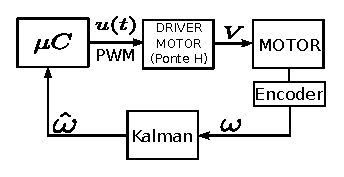
\includegraphics[width=0.5\textwidth]{figuras/ilustracoes/sistema_de_controle_embarcado.eps}
    \caption{Diagrama simplificado do sistema de controle embarcado para um motor.}
\end{figure}

\end{frame}

% Metodologia
\section{Metodologia}
\subsection{Robô}

\begin{frame}{Os Robôs}

\begin{itemize}
    \item Robôs que devem caber em um cubo com 7.5cm de lado;
    \item Microcontrolador: ESP32;
    \item Sensores: \emph{Encoder} magnéticos de $3$ pulsos por revolução (PPR).
\end{itemize}
    
    \begin{figure}
        \centering
        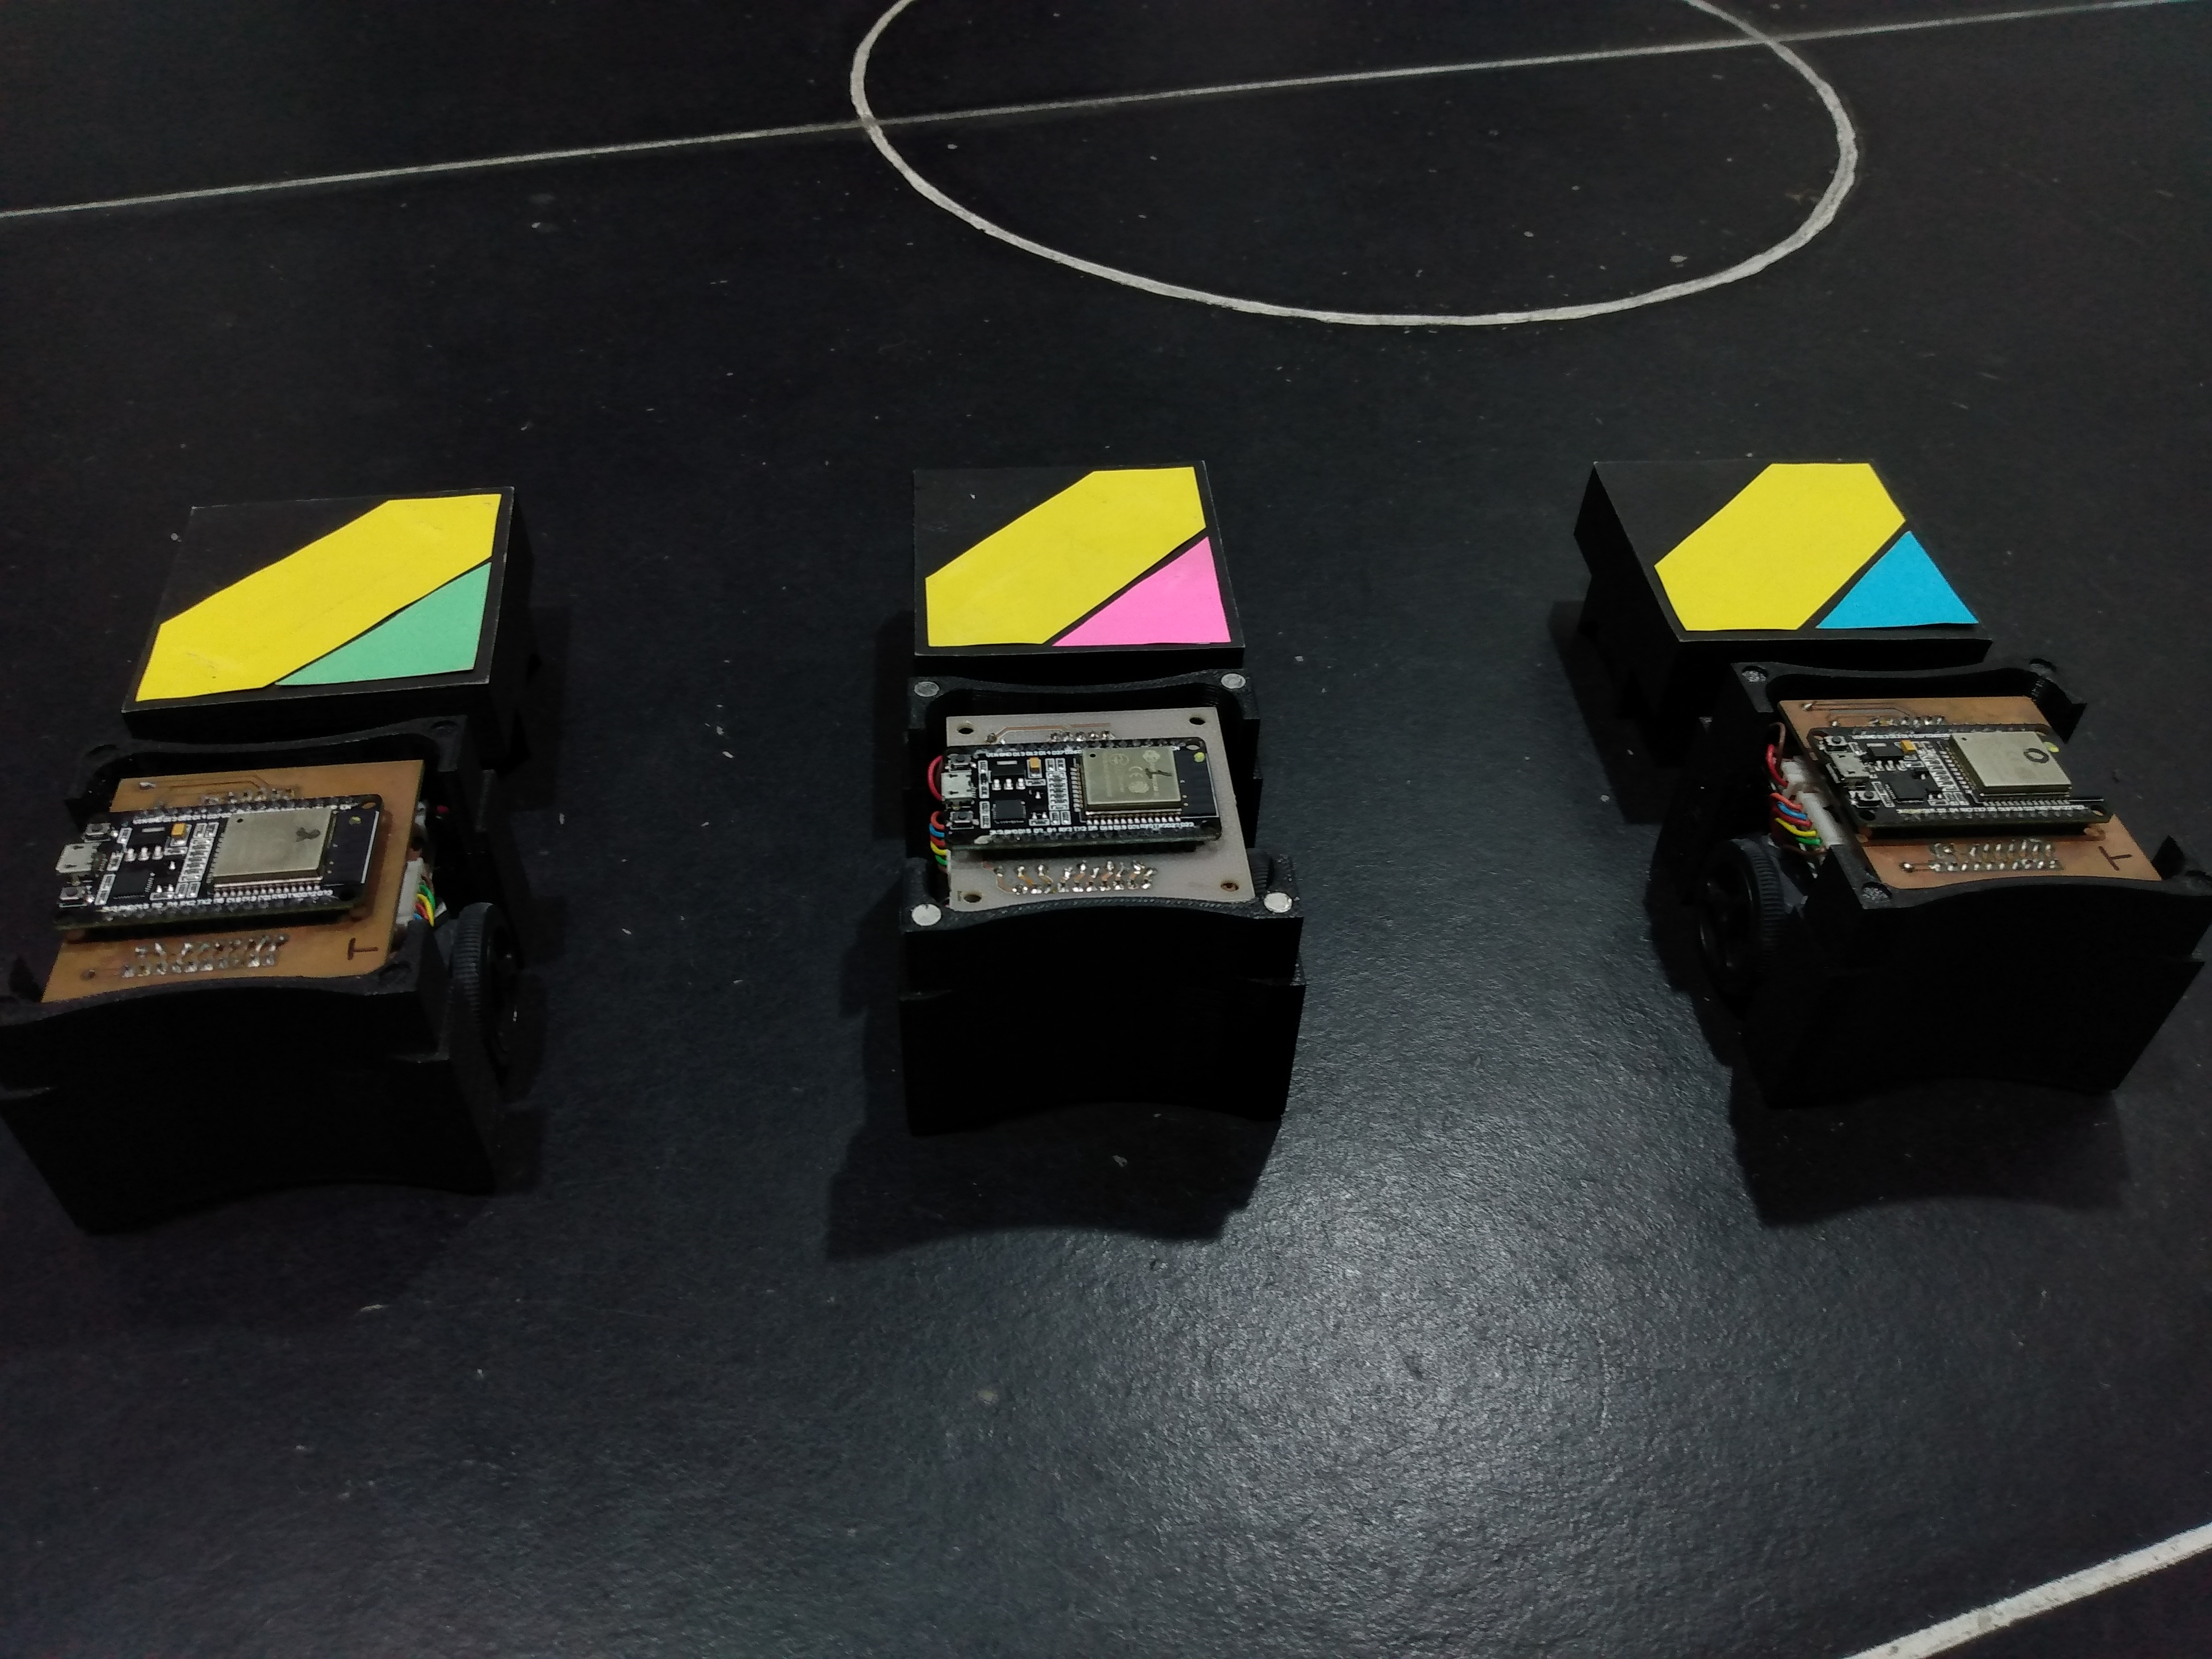
\includegraphics[width=0.4\textwidth]{figuras/robos/robos_capa_aberta.jpg}
        \caption{Robôs da Equipe POTI.}
    \end{figure}
\end{frame}


\begin{frame}{Projeto do Robô}
    \begin{figure}
        \centering
        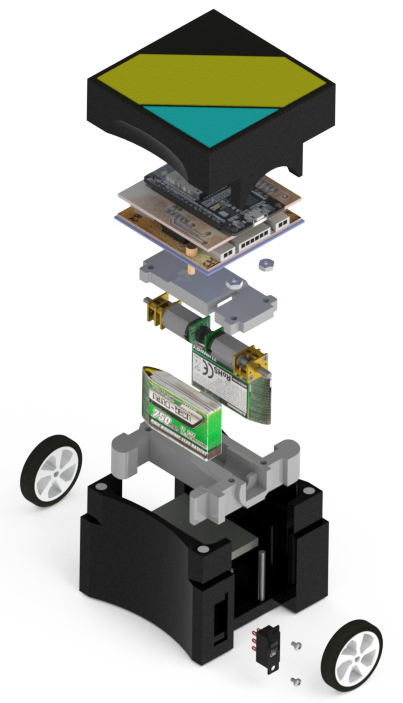
\includegraphics[width=0.25\textwidth ]{figuras/robos/robo_completo_explodido.png}
        \caption{Visão geral do projeto dos robôs utilizados.}
    \end{figure}
\end{frame}

\begin{frame}{O Microcontrolador}

\begin{itemize}
    \item CPUs: 2 núcleos principais e um terceiro núcleo de baixo consumo enérgico. 
    \item Frequência de operação dos núcleos: Até $240$ MHz
    \item Interface \emph{Wireless}: Wi-Fi e Bluetooth (802.11 b/g/n/e/i);
    \item Memória: 448 Kb de ROM, 520 Kb de SRAM e 4 Mb de Flash.
\end{itemize}

\begin{figure}[H]
    \centering
    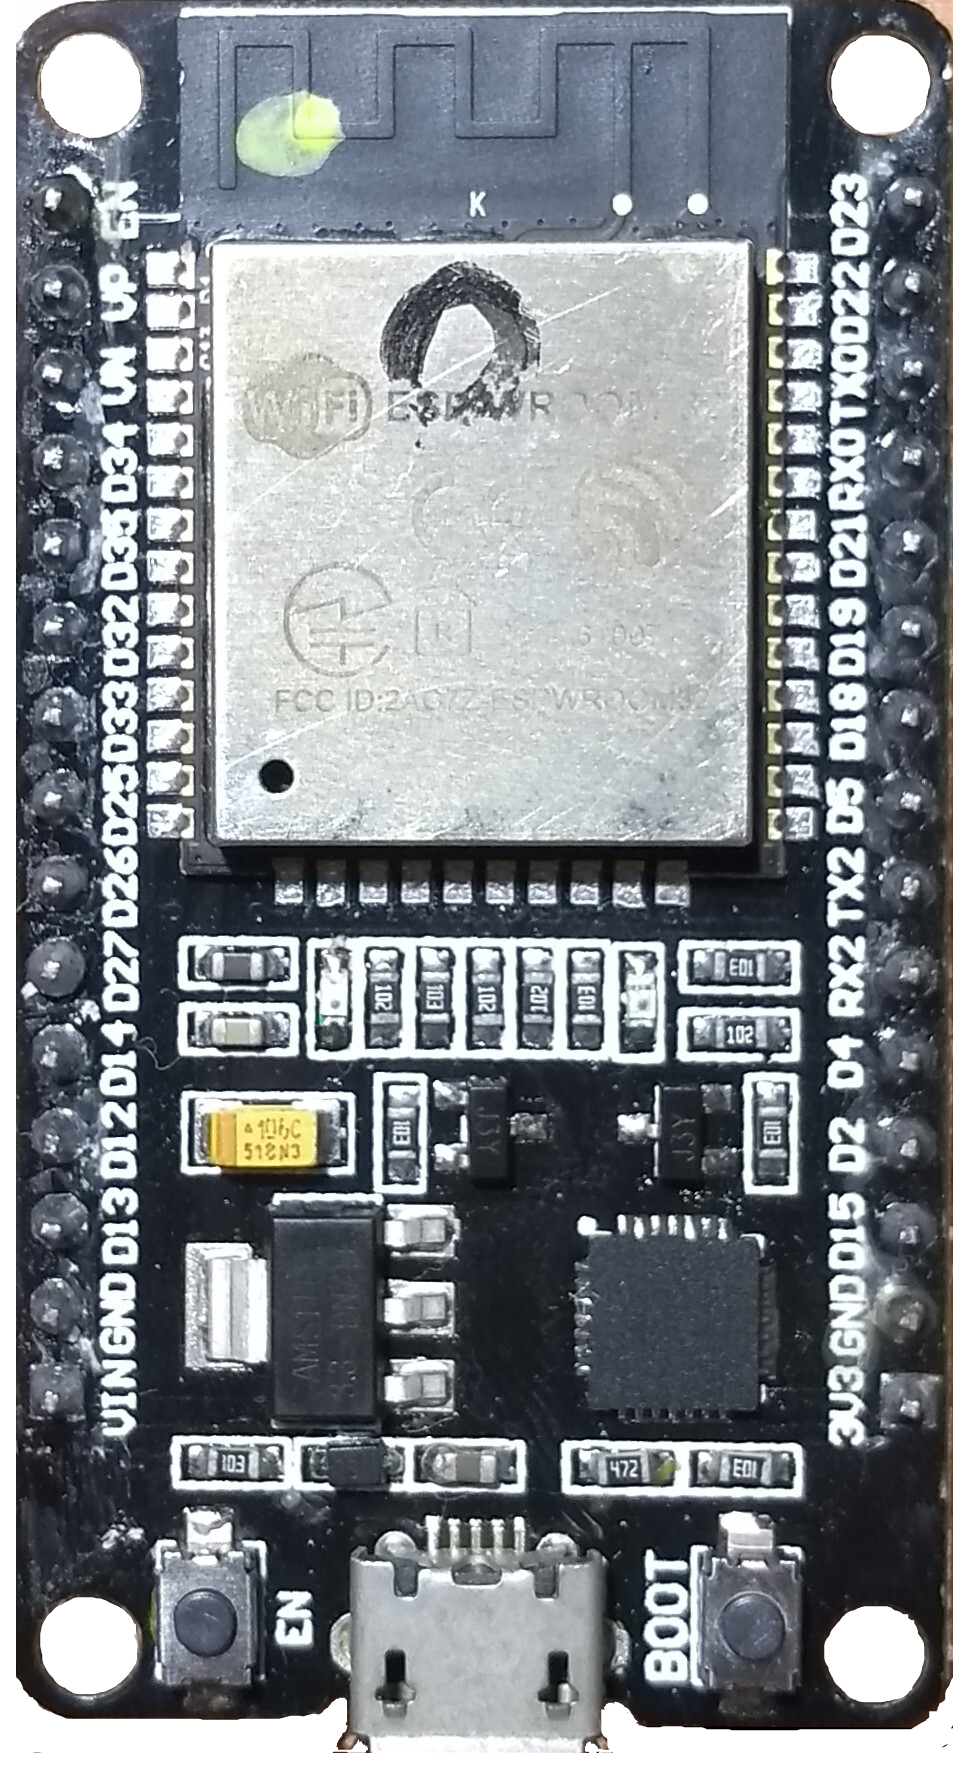
\includegraphics[width=0.1\textwidth]{figuras/eletronica/esp32_kit.png}
    \caption{Placa de desenvolvimento ESP32 Dev1.}
\end{figure}

\end{frame}

\begin{frame}{Conjunto Motor-Sensor}
    \begin{figure}
        \centering
        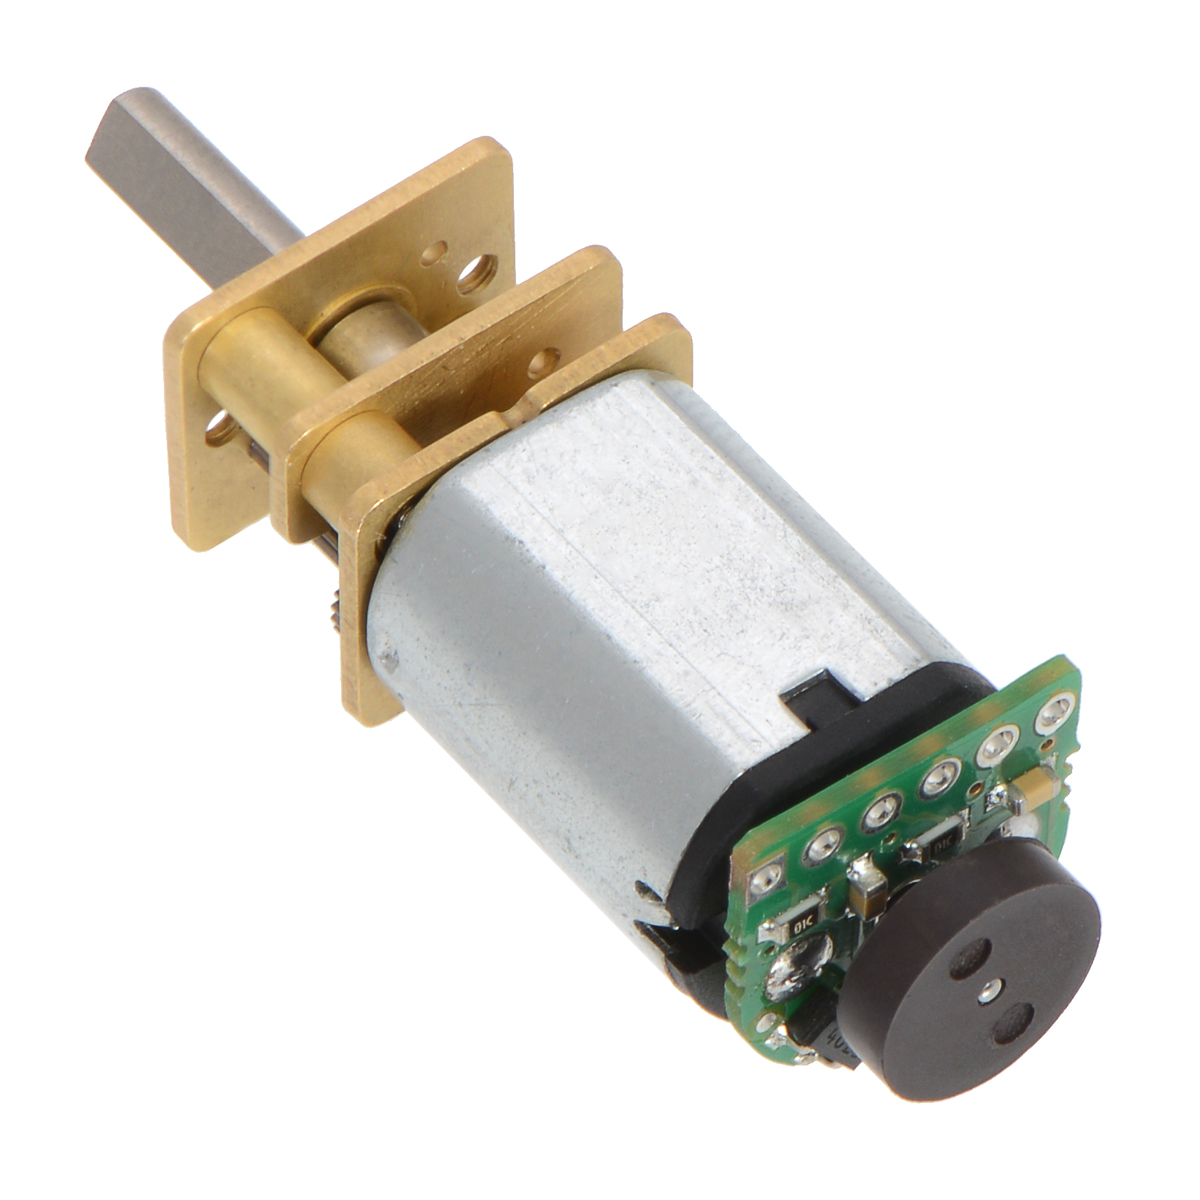
\includegraphics[width=0.4\textwidth]{figuras/eletronica/motor_com_encoder.jpg}
        \caption{Motor equipado com \emph{Encoder} magnético e caixa de redução de 30:1.}
    \end{figure}
\end{frame}

\subsection{\emph{Firmware}}
% \subsubsection{Comunicação}
\begin{frame}{Divisão de Tarefas no $\mu{}C$}
    \begin{figure}
        \centering
        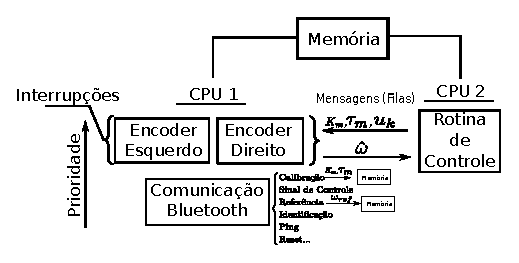
\includegraphics[width=1.0\textwidth]{figuras/ilustracoes/visao_geral_do_sistema.eps}
        \caption{Visão geral do sistema embarcado.}
    \end{figure}
\end{frame}

\begin{frame}{Rotina de Comunicação}
    
    \begin{figure}
        \centering
        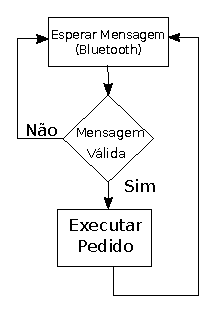
\includegraphics{figuras/ilustracoes/ilustracao_rotina_de_comunicacao.eps}
        \caption{Fluxo grama simplificado da rotina de comunicação.}
    \end{figure}
        
\end{frame}

\begin{frame}{Mensagem}
    \begin{figure}
        \centering
        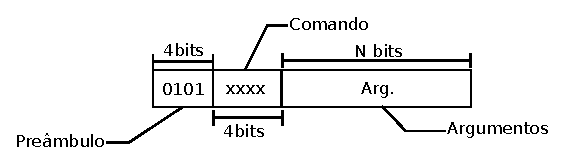
\includegraphics[width=1.0\textwidth]{figuras/ilustracoes/ilustracao_frame_generico.eps}
        \caption{Ilustração de um pacote genérico.}
    \end{figure}
\end{frame}

\begin{frame}{Comandos}
    \begin{align*}
    \text{Comandos}
        \begin{cases}
            \text{Pedir dados da Calibração:} & 0000\\
            \text{Realizar Calibração:} & 0100\\
            \text{Velocidades de Referência:} & 1010\\
            \text{Sinal de Controle:} & 1011\\
            \text{Velocidades Atuais:} & 0011\\
            \text{Iniciar rotina de coleta de dados(\emph{Identify}):} & 0101\\
            \text{Teste de conexão (\emph{Ping}):} & 1111
        \end{cases}
    \end{align*}
\end{frame}

\begin{frame}{Comando:Referência}
    \begin{figure}
        \centering
        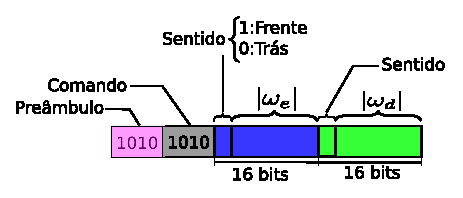
\includegraphics[width=\textwidth]{figuras/ilustracoes/ilustracao_comando_omega_ref.eps}
        \caption{Telecomando de velocidades de referência.}
    \end{figure}
\end{frame}

\begin{frame}{Comando:Sinal de Controle}
    \begin{figure}
        \centering
        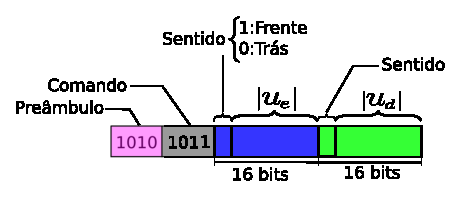
\includegraphics[width=\textwidth]{figuras/ilustracoes/ilustracao_comando_sinal_de_controle.eps}
        \caption{Telecomando de sinal de controle.}
    \end{figure}
\end{frame}

\begin{frame}{Comando:Coleta de Dados}
    \begin{figure}
        \centering
        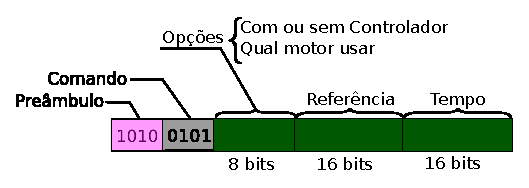
\includegraphics[width=\textwidth]{figuras/ilustracoes/ilustracao_comando_coleta_de_dados.eps}
        \caption{Telecomando para coleta de dados.}
    \end{figure}
\end{frame}
% \subsubsection{Calibração}
\begin{frame}{Rotina de Calibração}
    
    \begin{figure}
        \centering
        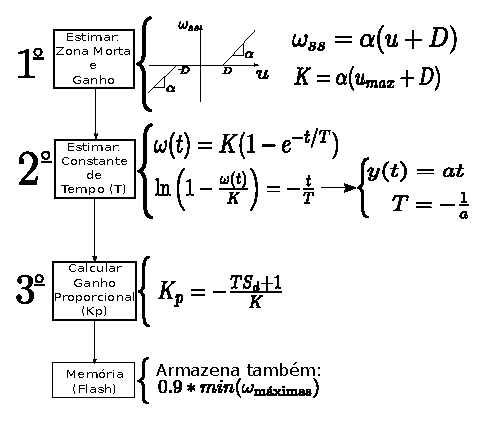
\includegraphics[width=0.5\textwidth]{figuras/ilustracoes/rotina_de_calibracao.eps}
        \caption{Visão geral da função de calibração.}
    \end{figure}
    
\end{frame}
% \subsubsection{Leitura dos Sensores}
\begin{frame}{Rotina de Leitura dos Sensores}
    ...    
\end{frame}
% \subsubsection{Rotina de Controle}

\begin{frame}{Rotina de Controle}
    ...    
\end{frame}


\subsection{Experimentos e Validação}
\begin{frame}{Experimentos e Validação}
    
\end{frame}



% Resultados
\section{Resultados}

\begin{frame}{Resultados}
    % Please add the following required packages to your document preamble:
% \usepackage{graphicx}
\begin{table}[H]
\centering
\resizebox{\textwidth}{!}{%
\begin{tabular}{c|cc|cc|cc|cc}
\multicolumn{1}{r|}{\textbf{}} &
  \multicolumn{2}{c|}{\textbf{$K_m$ {[}rad/s{]}}} &
  \multicolumn{2}{c}{\textbf{$\tau_m$ {[}s{]}}} &
  \multicolumn{2}{c|}{\textbf{$K_p$ {[}$1/(rad/s)${]}}} \\
\textbf{Experimento} &
  \textbf{\begin{tabular}[c]{@{}c@{}}Motor\\ Esquerdo\end{tabular}} &
  \textbf{\begin{tabular}[c]{@{}c@{}}Motor\\ Direito\end{tabular}} &
  \textbf{\begin{tabular}[c]{@{}c@{}}Motor\\ Esquerdo\end{tabular}} &
  \textbf{\begin{tabular}[c]{@{}c@{}}Motor\\ Direito\end{tabular}} &
  \textbf{\begin{tabular}[c]{@{}c@{}}Motor\\ Esquerdo\end{tabular}} &
  \textbf{\begin{tabular}[c]{@{}c@{}}Motor\\ Direito\end{tabular}} \\ \hline
\textbf{1} &
  3236.80 &
  3047.72 &
  7.62e-02 &
  6.57e-02 &
  1.37e-04 &
  1.24e-04 \\
\textbf{2} &
  4446.69 &
  4514.56 &
  5.71e-02 &
  5.40e-02 &
  3.01e-05 &
  3.23e-05 \\
\textbf{3} &
  4335.81 &
  4394.23 &
  5.48e-02 &
  5.30e-02 &
  1.54e-05 &
  2.11e-05 \\
\textbf{4} &
  3345.83 &
  3644.55 &
  4.43e-02 &
  5.90e-02 &
  5.55e-05 &
  3.80e-05
\end{tabular}%
}
\caption{Resultado da calibração para os diferentes experimentos.}
\label{tab:resumo_calibracao}
\end{table}
\end{frame}

\subsection{Experimento 01}
\begin{frame}{Resultado da Calibração}

\begin{figure}
    \begin{subfigure}{.45\textwidth}
    \centering
        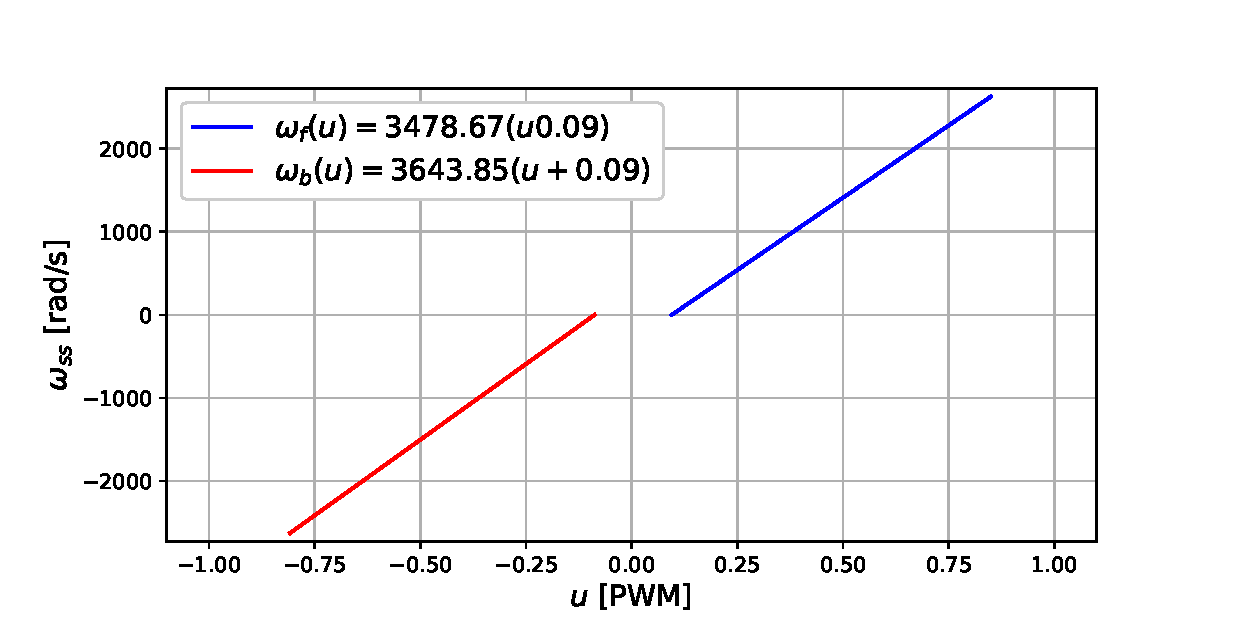
\includegraphics[width=\textwidth]{figuras/resultados/exp01/curva_feedforward_esquerdo100.eps}
        \caption{Motor esquerdo.}
    \end{subfigure}
    \begin{subfigure}{.45\textwidth}
        \centering
        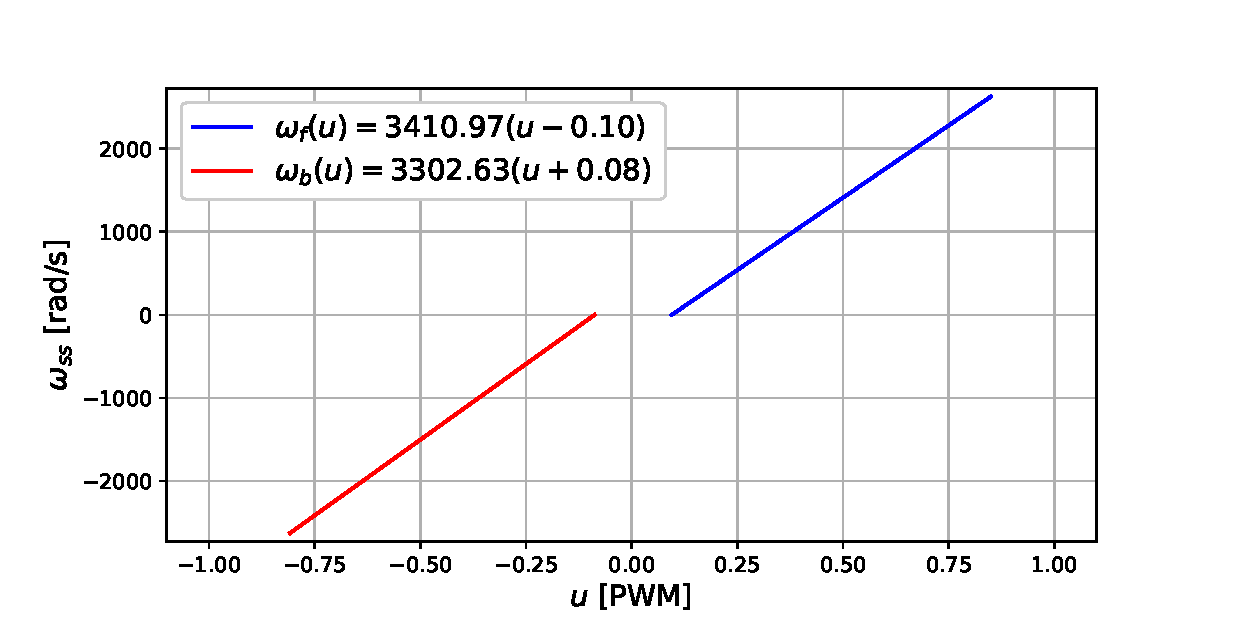
\includegraphics[width=\textwidth]{figuras/resultados/exp01/curva_feedforward_direito100.eps}
        \caption{Motor direito.}
    \end{subfigure}
    \caption{Curva $\omega_{ss}(u)$.}
\end{figure}

\end{frame}

\begin{frame}{Resultado da Aproximação do Comportamento do Sistema}


\begin{figure}
    \begin{subfigure}{.45\textwidth}
        \centering
        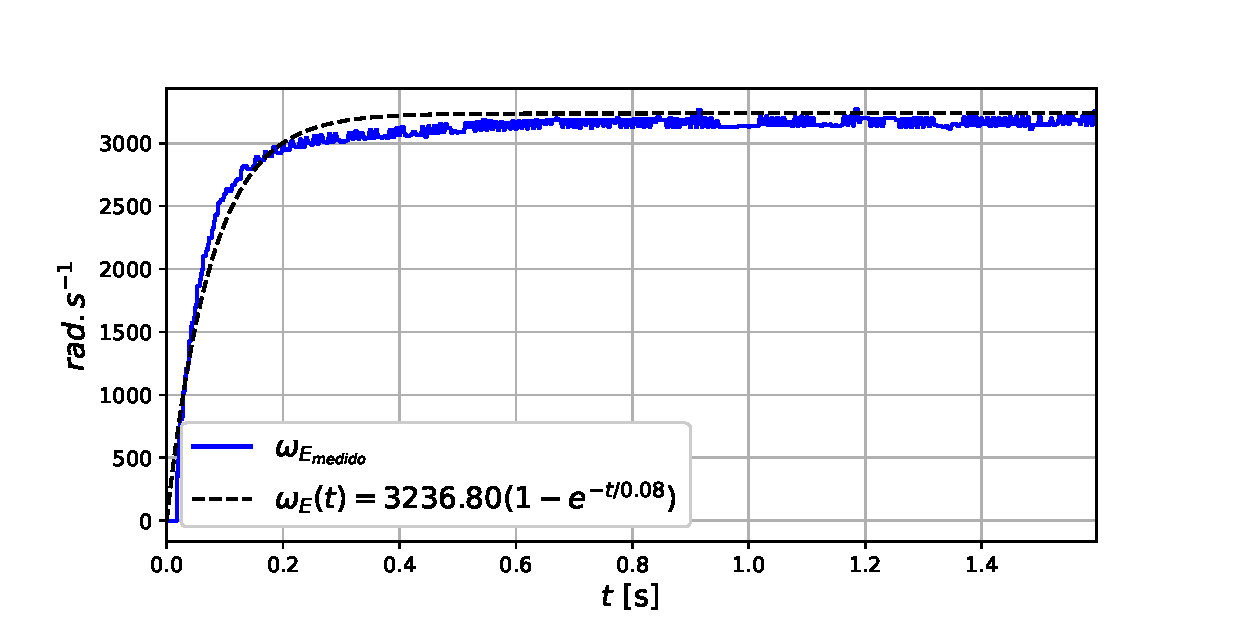
\includegraphics[width=\textwidth]{figuras/resultados/exp01/regressao_vs_medido_esquerdo100.eps}
        \caption{Motor Esquerdo.}
    \end{subfigure}
    \begin{subfigure}{.45\textwidth}
        \centering
        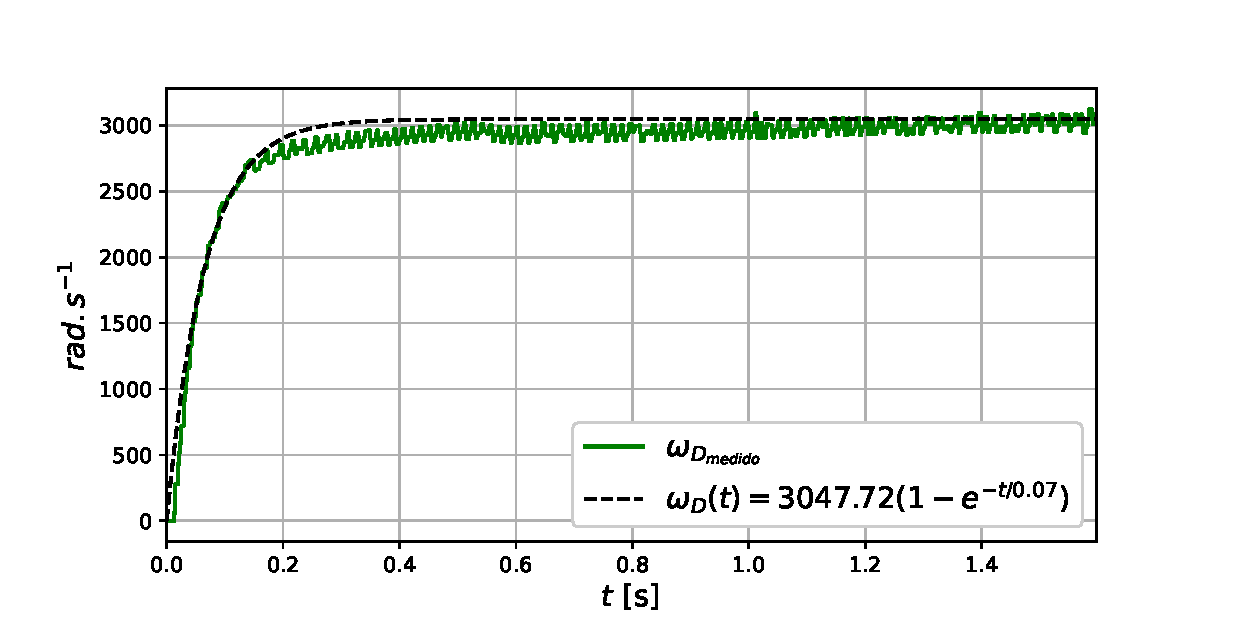
\includegraphics[width=\textwidth]{figuras/resultados/exp01/regressao_vs_medido_direito100.eps}
        \caption{Motor Direito.}
    \end{subfigure}
    \caption{Curva $\omega(t)$ teórica versus $\omega_{\text{medido}}$.}
\end{figure}
    
\end{frame}


\begin{frame}{Resultado da Filtragem}

    \begin{figure}
        \begin{subfigure}{.45\textwidth}
            \centering
            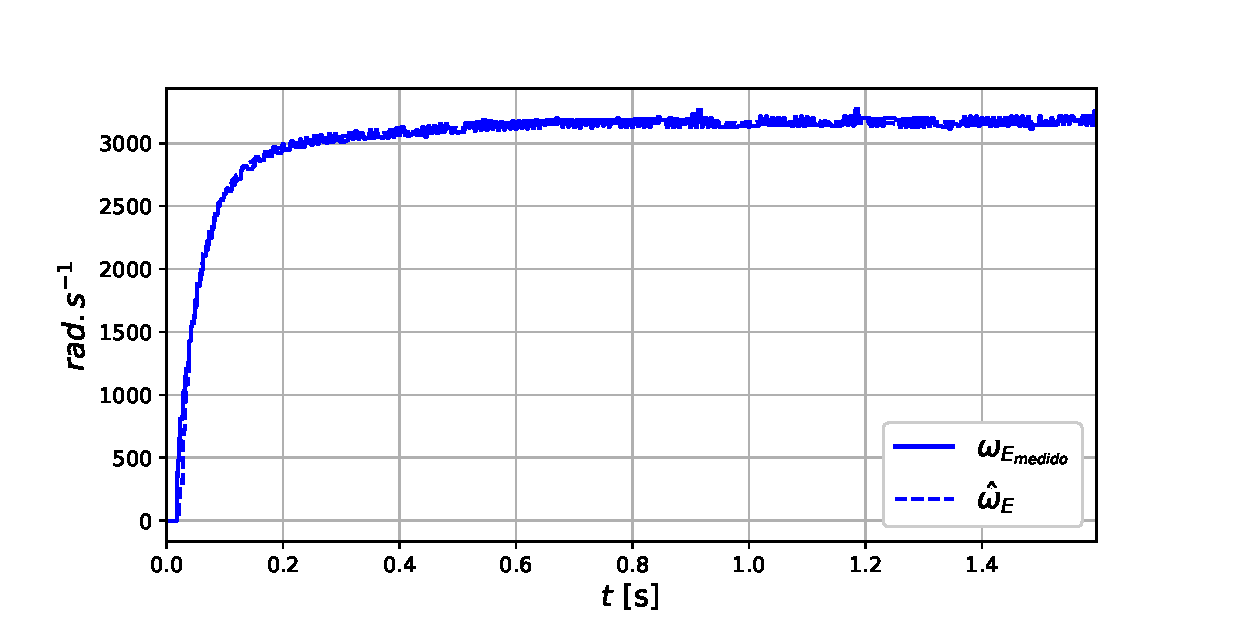
\includegraphics[width=\textwidth]{figuras/resultados/exp01/filtro_vs_sem_filtro_esquerdo100.eps}
            \caption{Motor Esquerdo.}
        \end{subfigure}
        \begin{subfigure}{.45\textwidth}
            \centering
            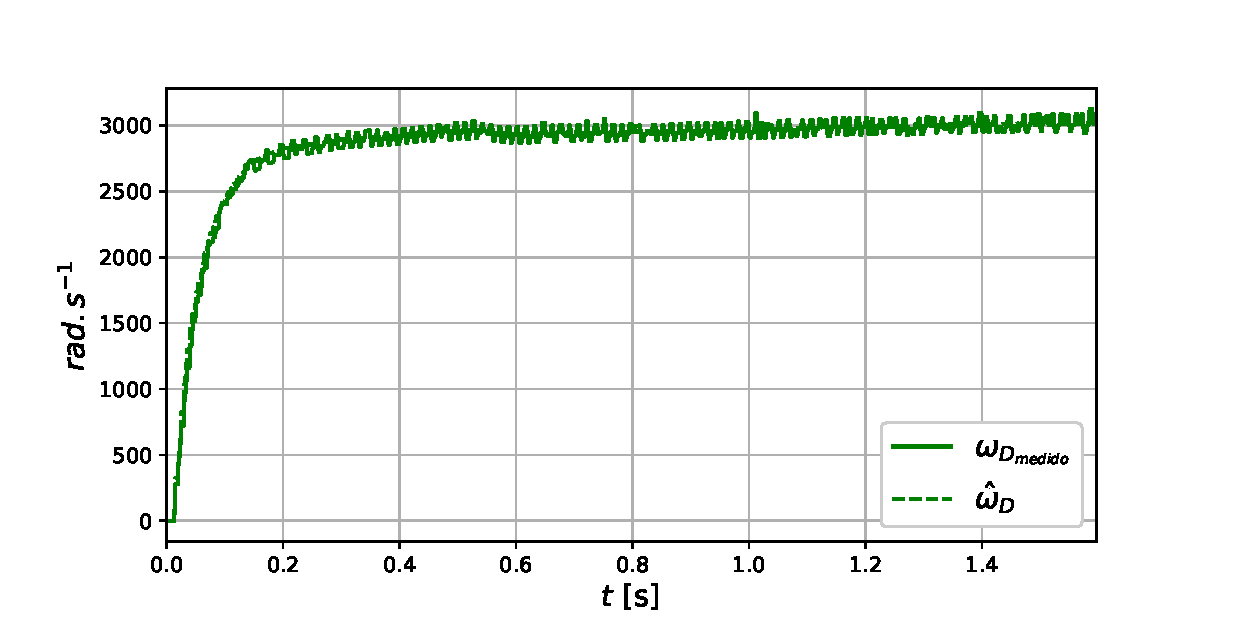
\includegraphics[width=\textwidth]{figuras/resultados/exp01/filtro_vs_sem_filtro_direito100.eps}
            \caption{Motor Direito.}
        \end{subfigure}
        \caption{Comparação entre a velocidade estimativa $\hat{\omega}$ e a velocidade $\omega$ medida.}
    \end{figure}
    
\end{frame}

\begin{frame}{Resultado do Controle}

    \begin{figure}
        \centering
        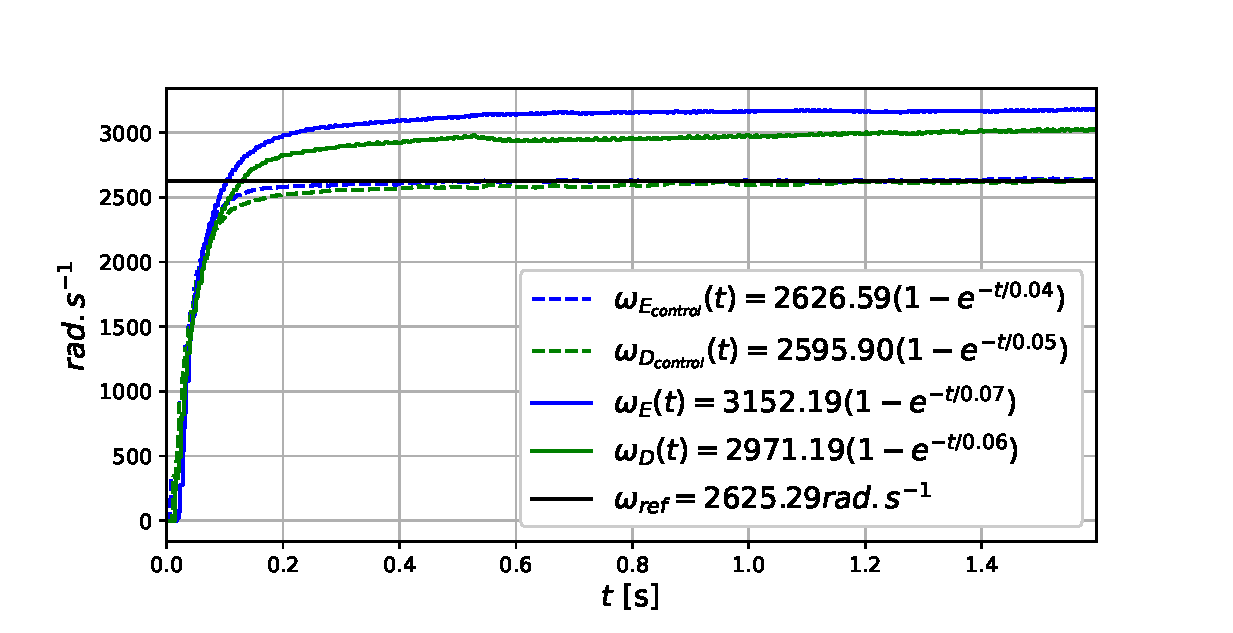
\includegraphics[width=0.6\textwidth]{figuras/resultados/exp01/controlador_vs_sem_controlador100.eps}
        \caption{Comparação entre o sistema com controlador e sem controlador.}
    \end{figure}
    
\end{frame}

\begin{frame}{Comparação}
    \begin{figure}
        \centering
        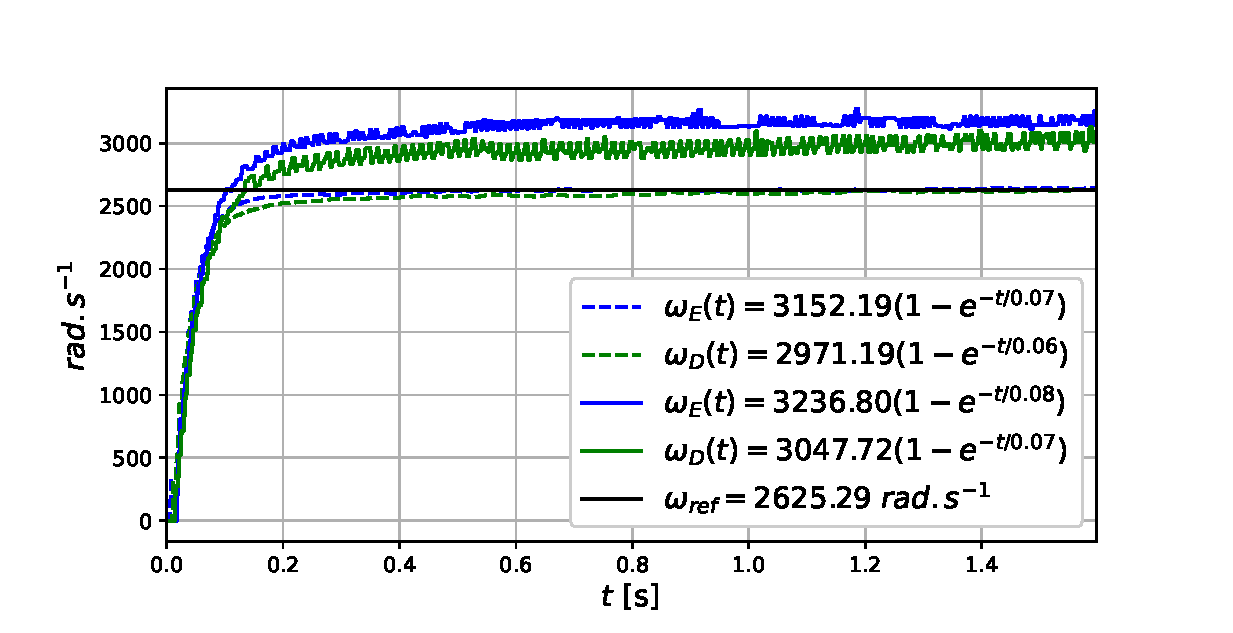
\includegraphics[width=0.6\textwidth]{figuras/resultados/exp01/antes_vs_depois100.eps}
        \caption{Resposta sem o filtro de \emph{kalman} e sem controle versus com controlador e com o filtro.}
    \end{figure}
\end{frame}
\subsection{Experimento 02}
\begin{frame}{Resultado da Calibração}

\begin{figure}
    \begin{subfigure}{.45\textwidth}
    \centering
        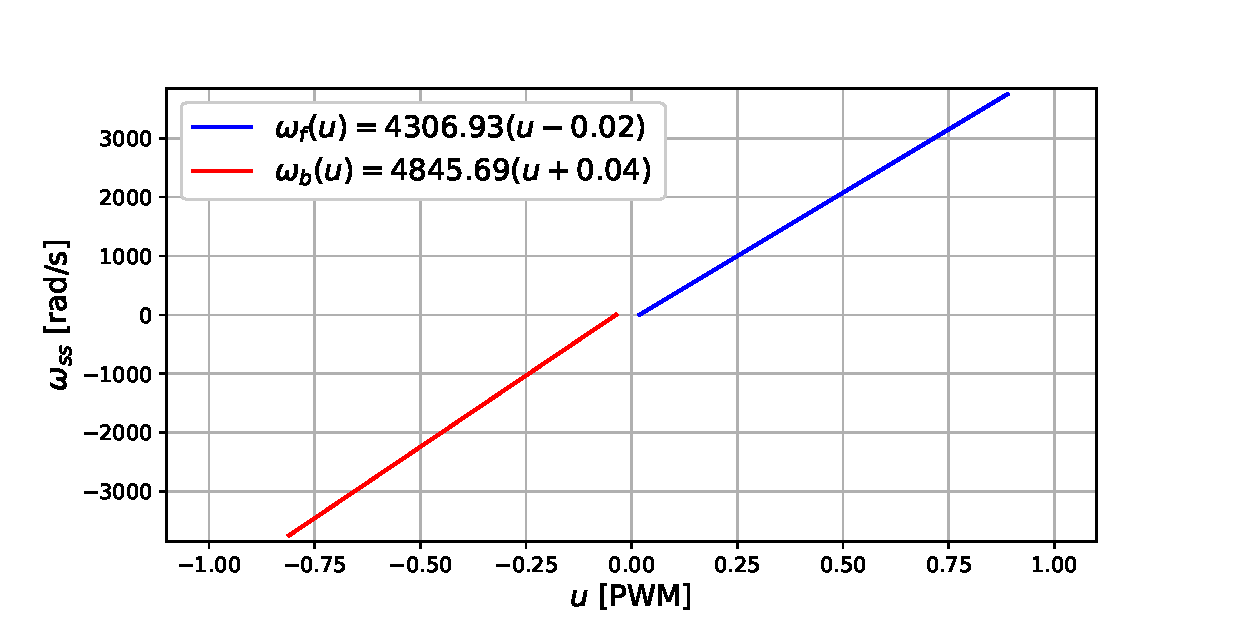
\includegraphics[width=\textwidth]{figuras/resultados/exp02/curva_feedforward_esquerdo100.eps}
        \caption{Motor esquerdo.}
    \end{subfigure}
    \begin{subfigure}{.45\textwidth}
        \centering
        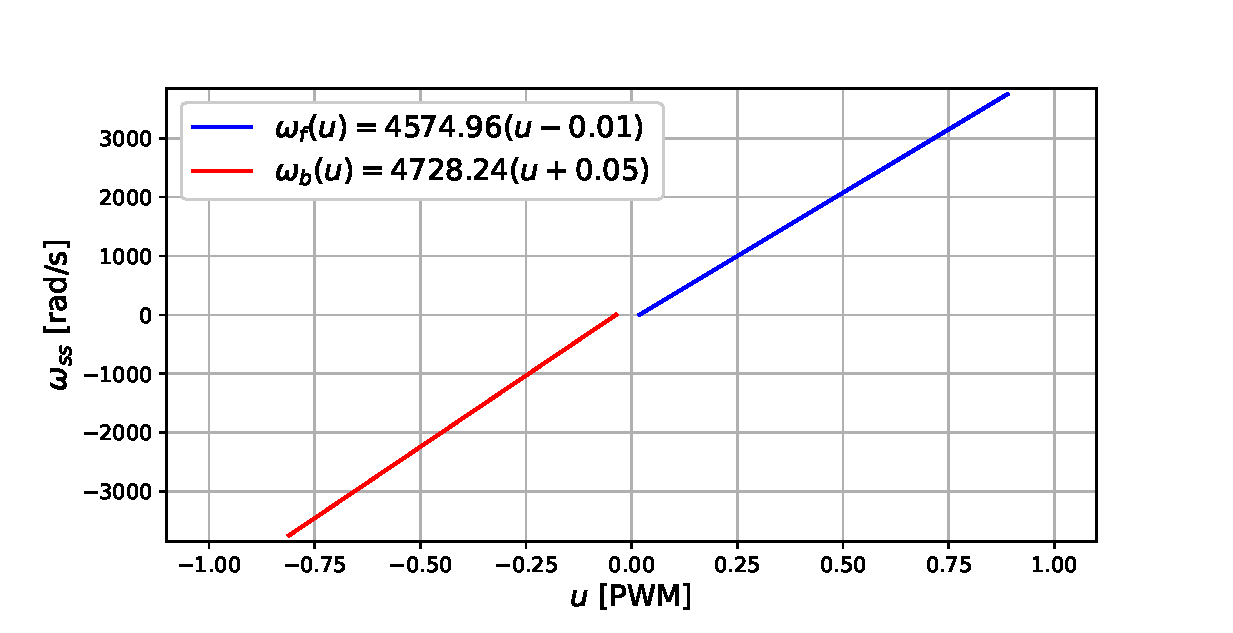
\includegraphics[width=\textwidth]{figuras/resultados/exp02/curva_feedforward_direito100.eps}
        \caption{Motor direito.}
    \end{subfigure}
    \caption{Curva $\omega_{ss}(u)$.}
\end{figure}

\end{frame}

\begin{frame}{Resultado da Aproximação do Comportamento do Sistema}


\begin{figure}
    \begin{subfigure}{.45\textwidth}
        \centering
        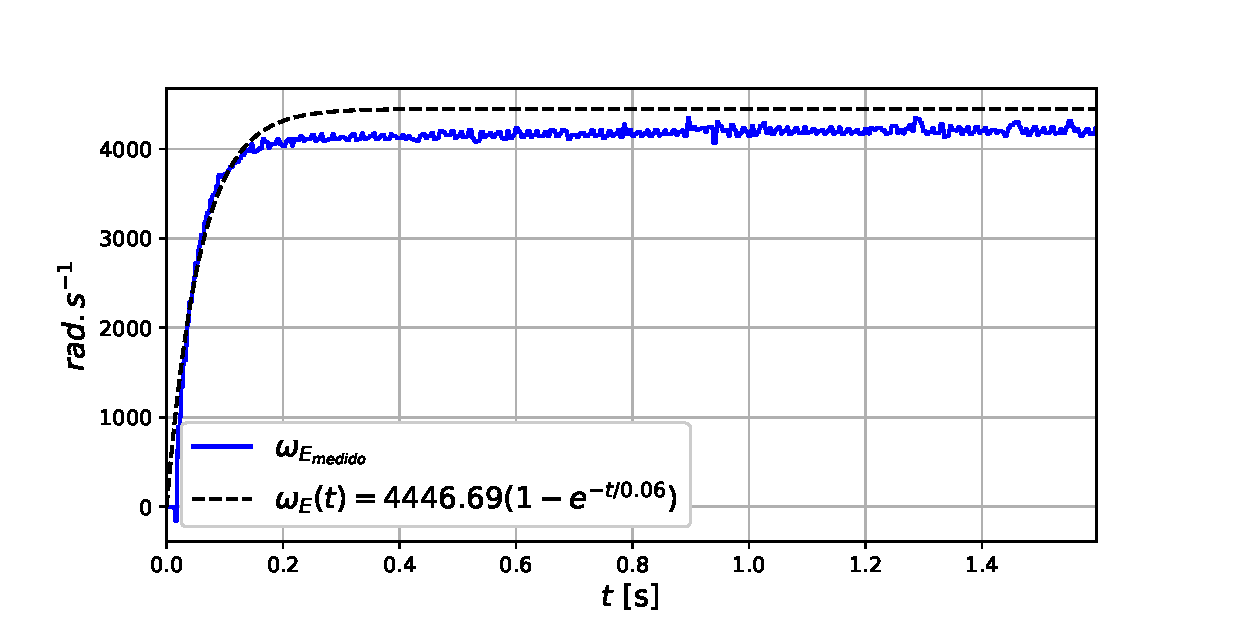
\includegraphics[width=\textwidth]{figuras/resultados/exp02/regressao_vs_medido_esquerdo100.eps}
        \caption{Motor Esquerdo.}
    \end{subfigure}
    \begin{subfigure}{.45\textwidth}
        \centering
        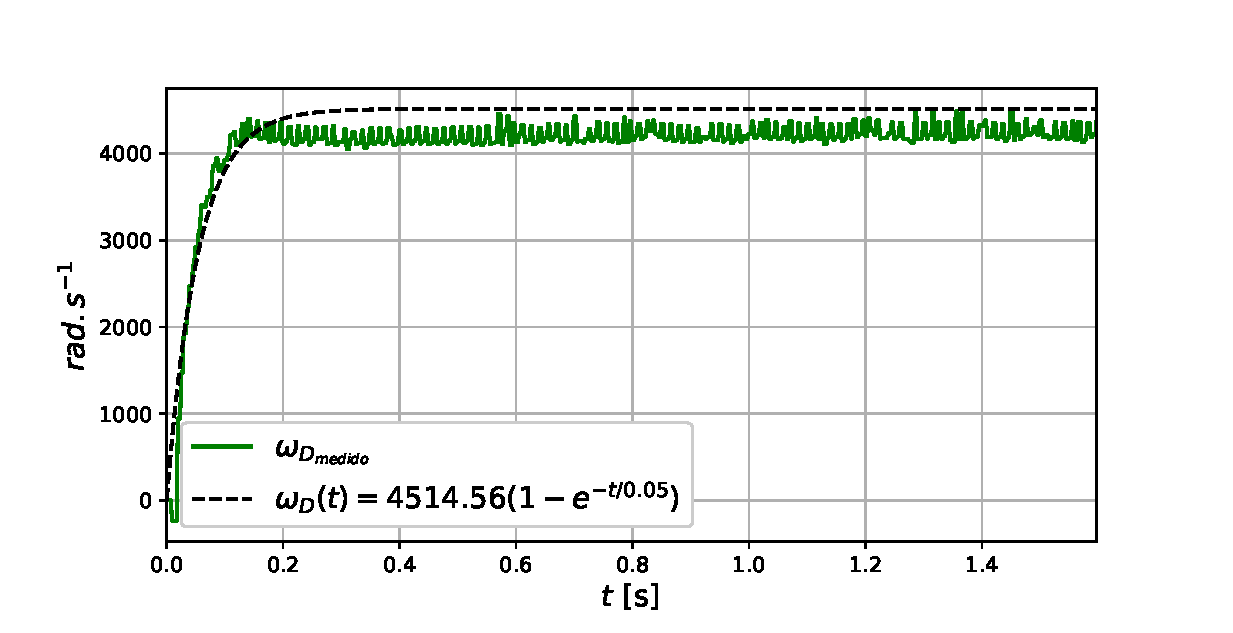
\includegraphics[width=\textwidth]{figuras/resultados/exp02/regressao_vs_medido_direito100.eps}
        \caption{Motor Direito.}
    \end{subfigure}
    \caption{Curva $\omega(t)$ teórica versus $\omega_{\text{medido}}$.}
\end{figure}
    
\end{frame}


\begin{frame}{Resultado da Filtragem}

    \begin{figure}
        \begin{subfigure}{.45\textwidth}
            \centering
            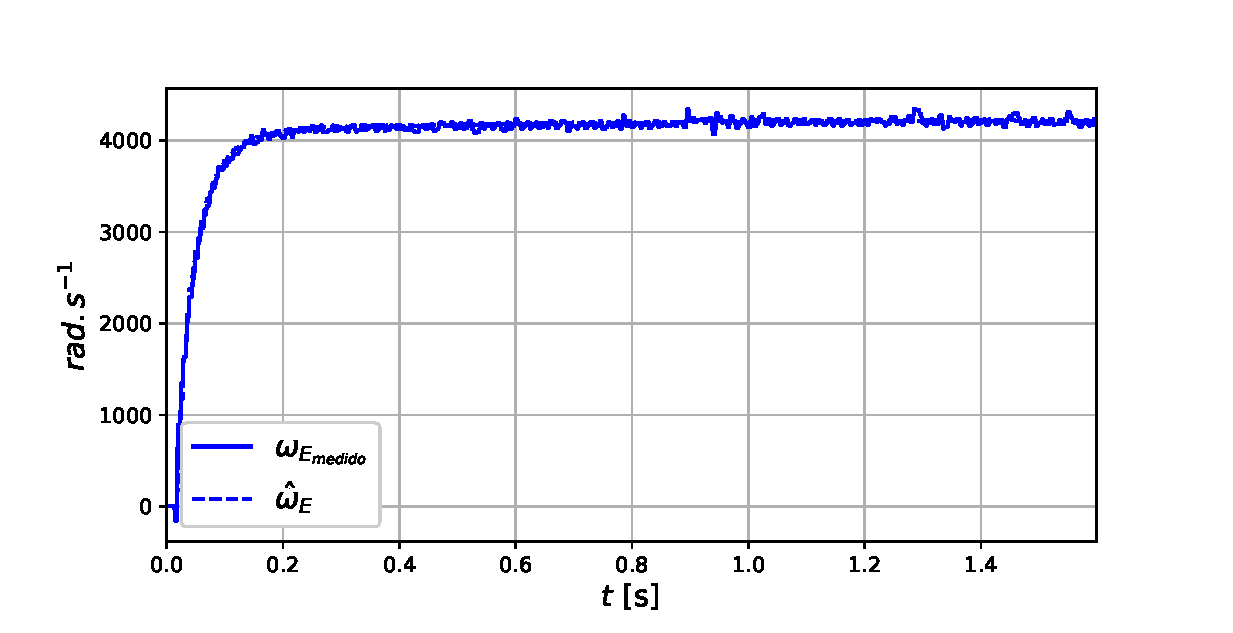
\includegraphics[width=\textwidth]{figuras/resultados/exp02/filtro_vs_sem_filtro_esquerdo100.eps}
            \caption{Motor Esquerdo.}
        \end{subfigure}
        \begin{subfigure}{.45\textwidth}
            \centering
            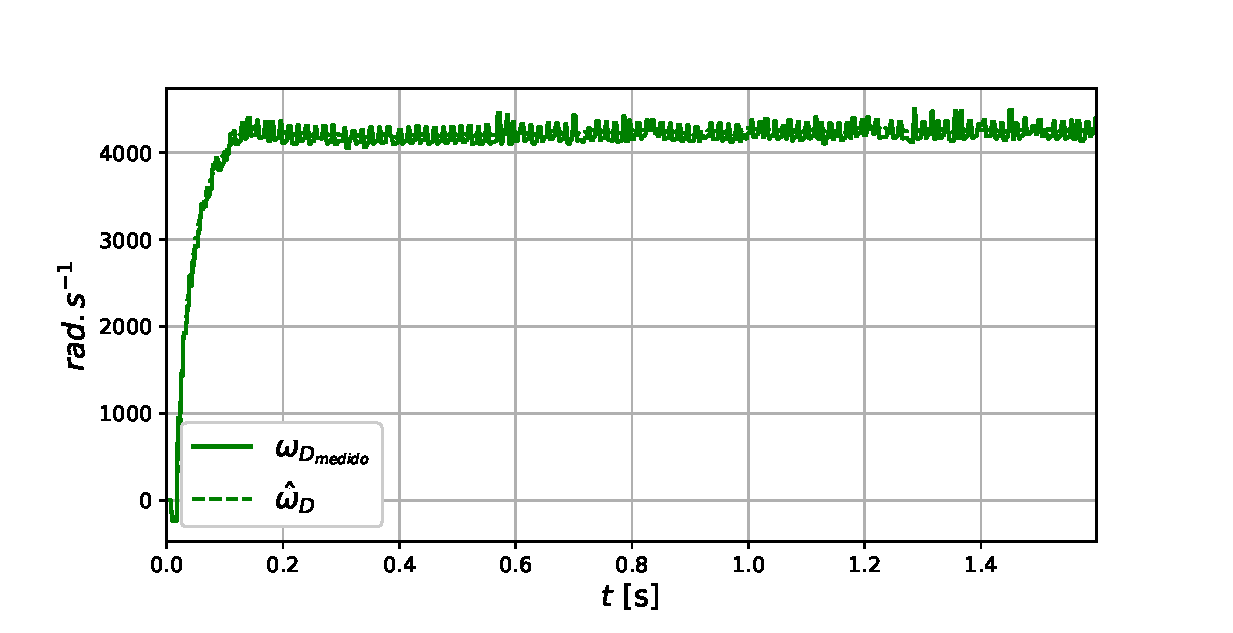
\includegraphics[width=\textwidth]{figuras/resultados/exp02/filtro_vs_sem_filtro_direito100.eps}
            \caption{Motor Direito.}
        \end{subfigure}
        \caption{Comparação entre a velocidade estimativa $\hat{\omega}$ e a velocidade $\omega$ medida.}
    \end{figure}
    
\end{frame}

\begin{frame}{Resultado do Controle}

    \begin{figure}
        \centering
        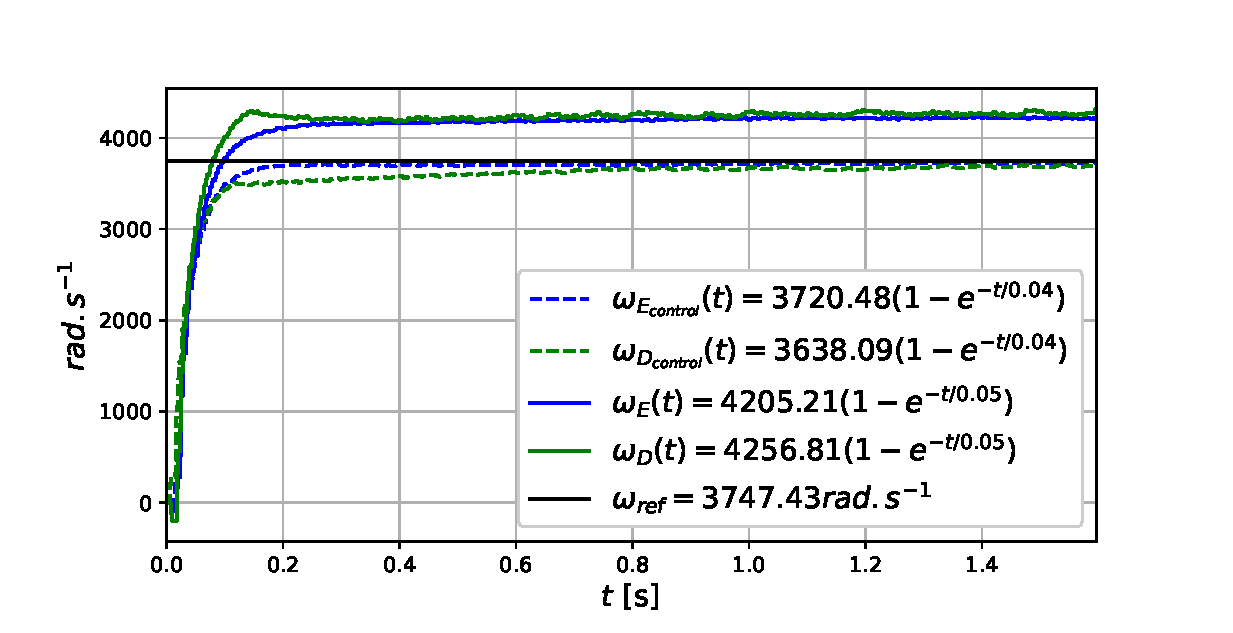
\includegraphics[width=0.6\textwidth]{figuras/resultados/exp02/controlador_vs_sem_controlador100.eps}
        \caption{Comparação entre o sistema com controlador e sem controlador.}
    \end{figure}
    
\end{frame}

\begin{frame}{Comparação}
    \begin{figure}
        \centering
        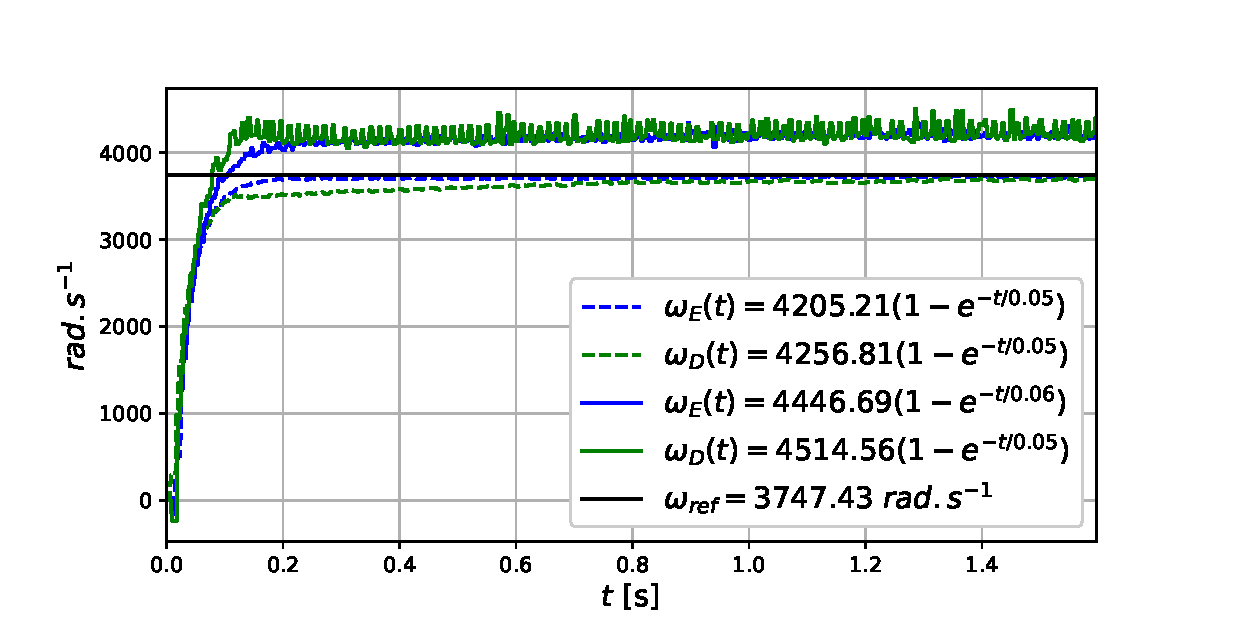
\includegraphics[width=0.6\textwidth]{figuras/resultados/exp02/antes_vs_depois100.eps}
        \caption{Resposta sem o filtro de \emph{kalman} e sem controle versus com controlador e com o filtro.}
    \end{figure}
\end{frame}
\subsection{Experimento 03}
\begin{frame}{Resultado da Calibração}

\begin{figure}
    \begin{subfigure}{.45\textwidth}
    \centering
        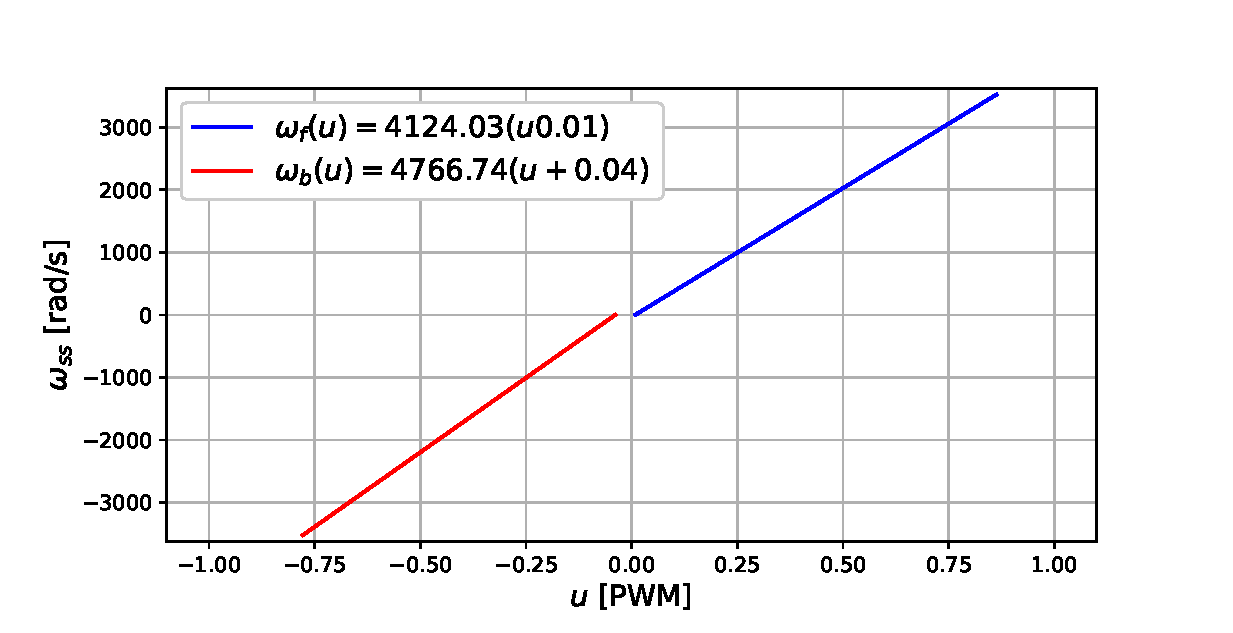
\includegraphics[width=\textwidth]{figuras/resultados/exp03/curva_feedforward_esquerdo100.eps}
        \caption{Motor esquerdo.}
    \end{subfigure}
    \begin{subfigure}{.45\textwidth}
        \centering
        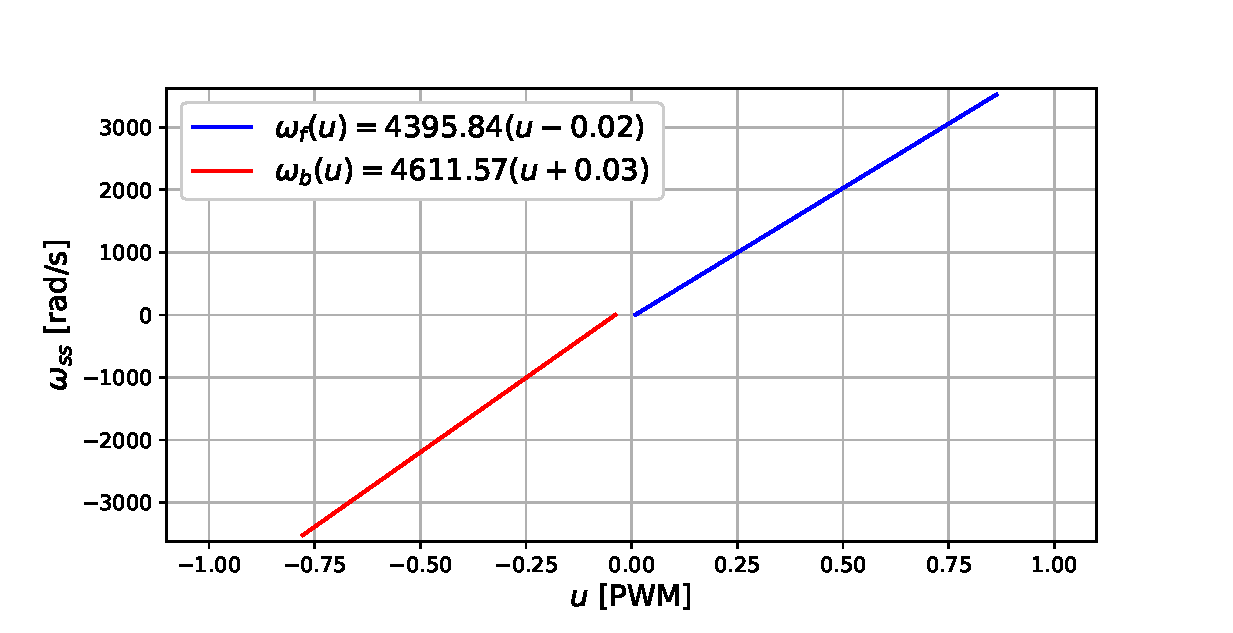
\includegraphics[width=\textwidth]{figuras/resultados/exp03/curva_feedforward_direito100.eps}
        \caption{Motor direito.}
    \end{subfigure}
    \caption{Curva $\omega_{ss}(u)$.}
\end{figure}

\end{frame}

\begin{frame}{Resultado da Aproximação do Comportamento do Sistema}


\begin{figure}
    \begin{subfigure}{.45\textwidth}
        \centering
        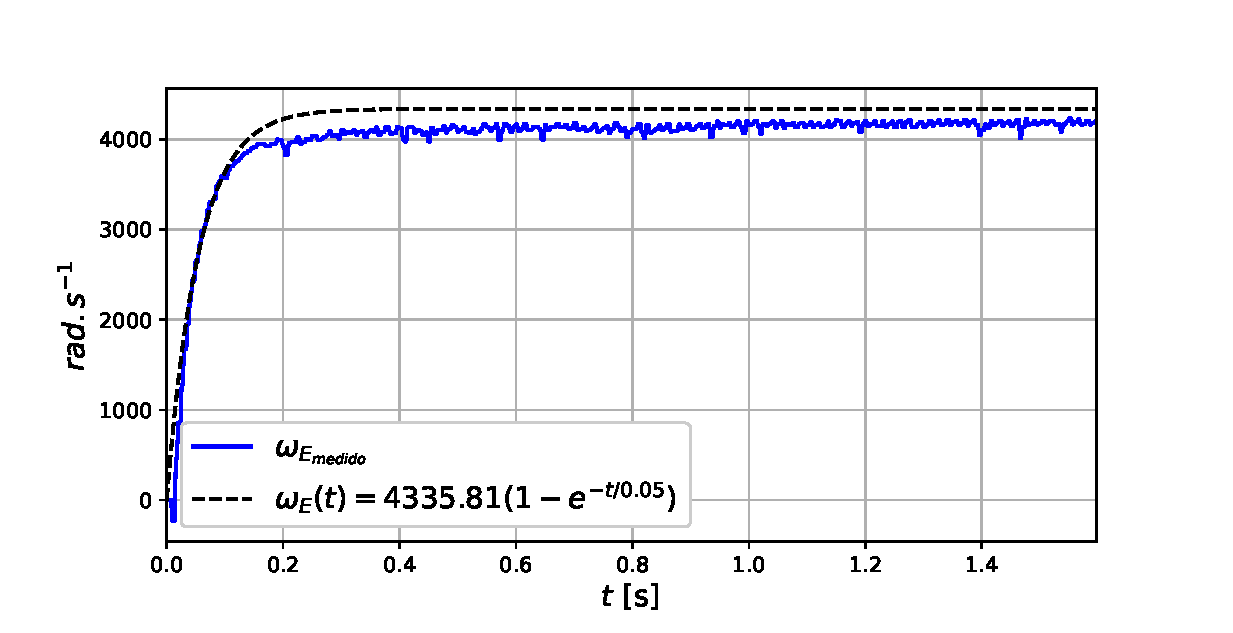
\includegraphics[width=\textwidth]{figuras/resultados/exp03/regressao_vs_medido_esquerdo100.eps}
        \caption{Motor Esquerdo.}
    \end{subfigure}
    \begin{subfigure}{.45\textwidth}
        \centering
        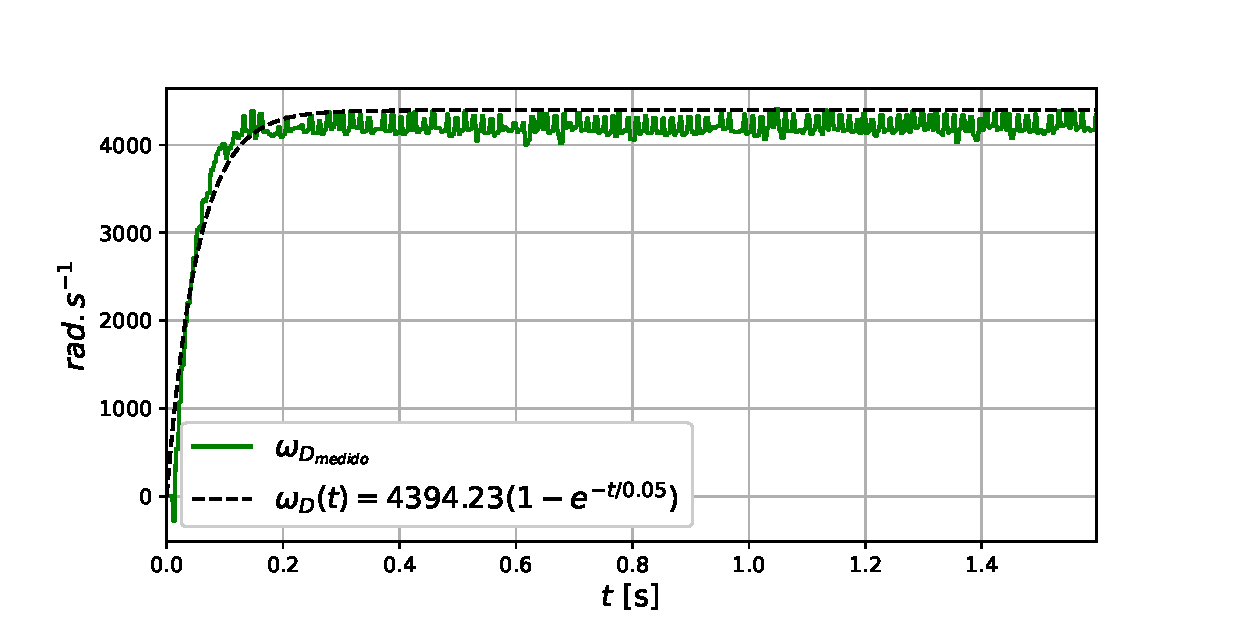
\includegraphics[width=\textwidth]{figuras/resultados/exp03/regressao_vs_medido_direito100.eps}
        \caption{Motor Direito.}
    \end{subfigure}
    \caption{Curva $\omega(t)$ teórica versus $\omega_{\text{medido}}$.}
\end{figure}
    
\end{frame}


\begin{frame}{Resultado da Filtragem}

    \begin{figure}
        \begin{subfigure}{.45\textwidth}
            \centering
            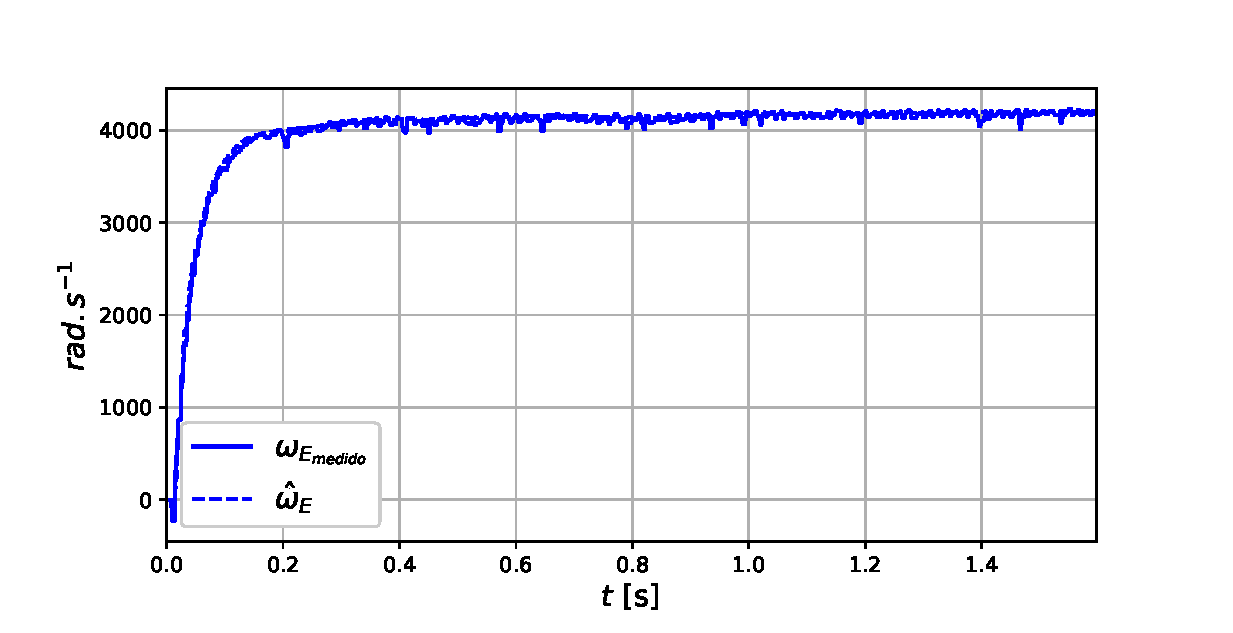
\includegraphics[width=\textwidth]{figuras/resultados/exp03/filtro_vs_sem_filtro_esquerdo100.eps}
            \caption{Motor Esquerdo.}
        \end{subfigure}
        \begin{subfigure}{.45\textwidth}
            \centering
            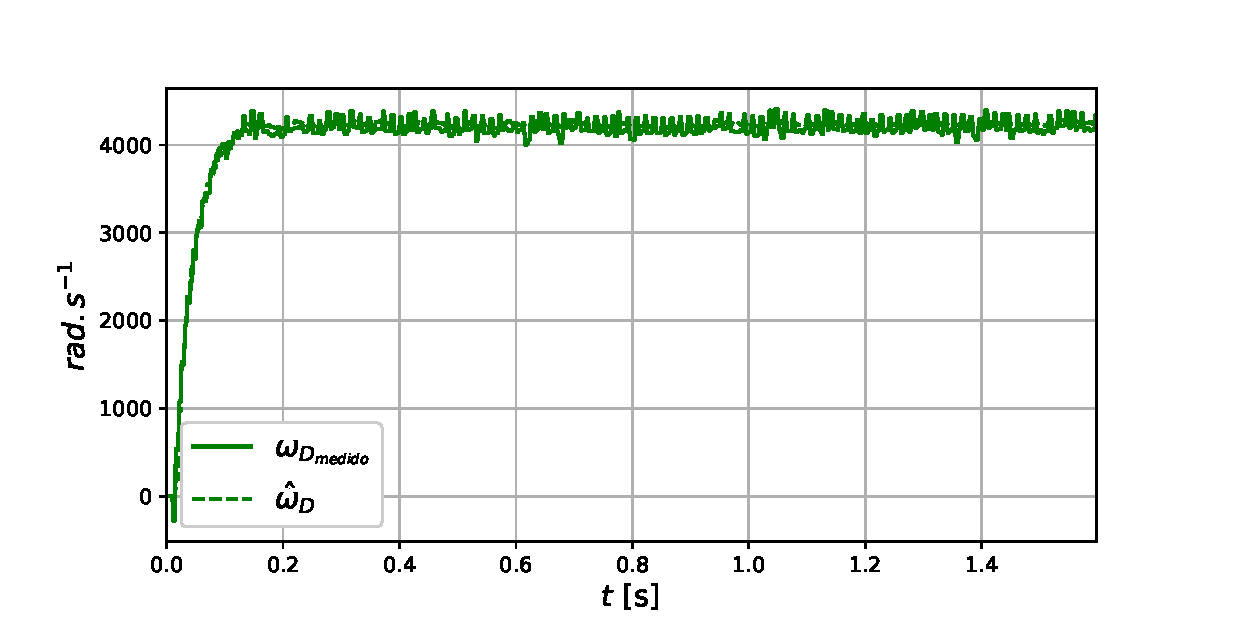
\includegraphics[width=\textwidth]{figuras/resultados/exp03/filtro_vs_sem_filtro_direito100.eps}
            \caption{Motor Direito.}
        \end{subfigure}
        \caption{Comparação entre a velocidade estimativa $\hat{\omega}$ e a velocidade $\omega$ medida.}
    \end{figure}
    
\end{frame}

\begin{frame}{Resultado do Controle}

    \begin{figure}
        \centering
        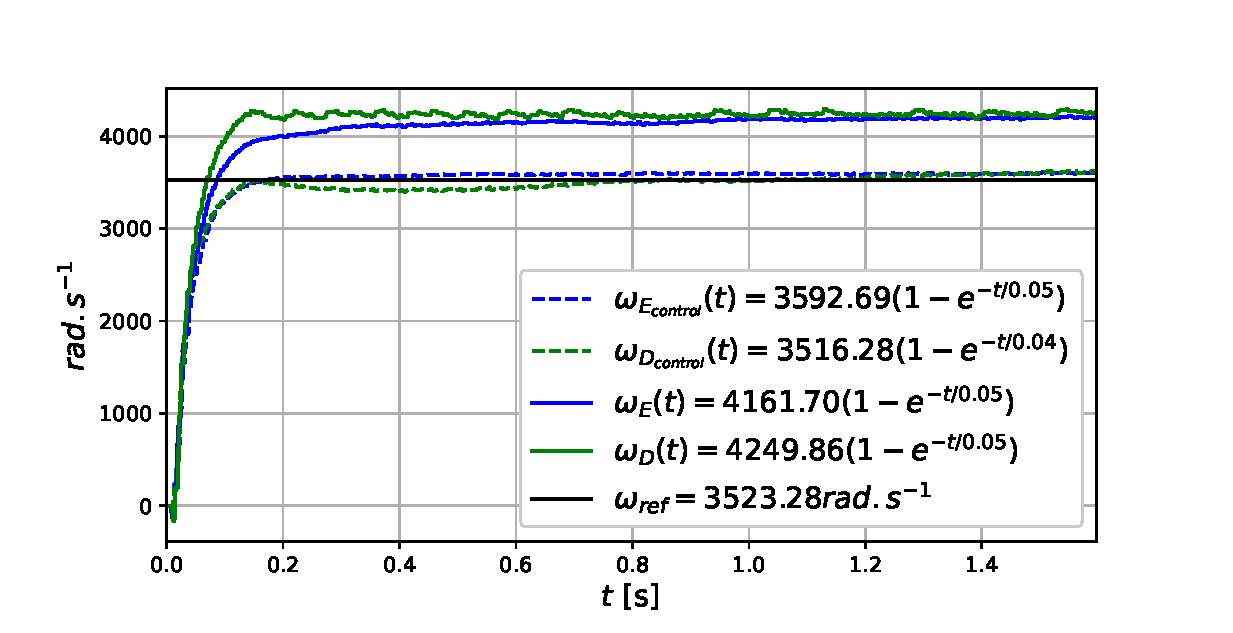
\includegraphics[width=0.6\textwidth]{figuras/resultados/exp03/controlador_vs_sem_controlador100.eps}
        \caption{Comparação entre o sistema com controlador e sem controlador.}
    \end{figure}
    
\end{frame}

\begin{frame}{Comparação}
    \begin{figure}
        \centering
        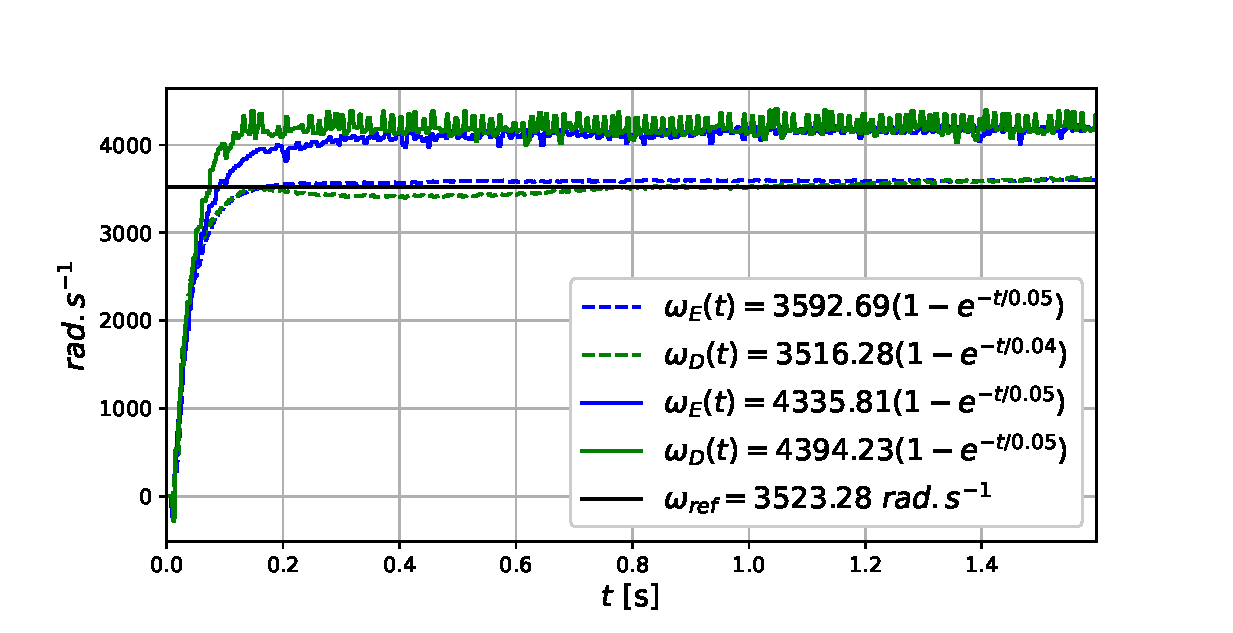
\includegraphics[width=0.6\textwidth]{figuras/resultados/exp03/antes_vs_depois100.eps}
        \caption{Resposta sem o filtro de \emph{kalman} e sem controle versus com controlador e com o filtro.}
    \end{figure}
\end{frame}
\subsection{Experimento 04}
\begin{frame}{Resultado da Calibração}

\begin{figure}
    \begin{subfigure}{.45\textwidth}
    \centering
        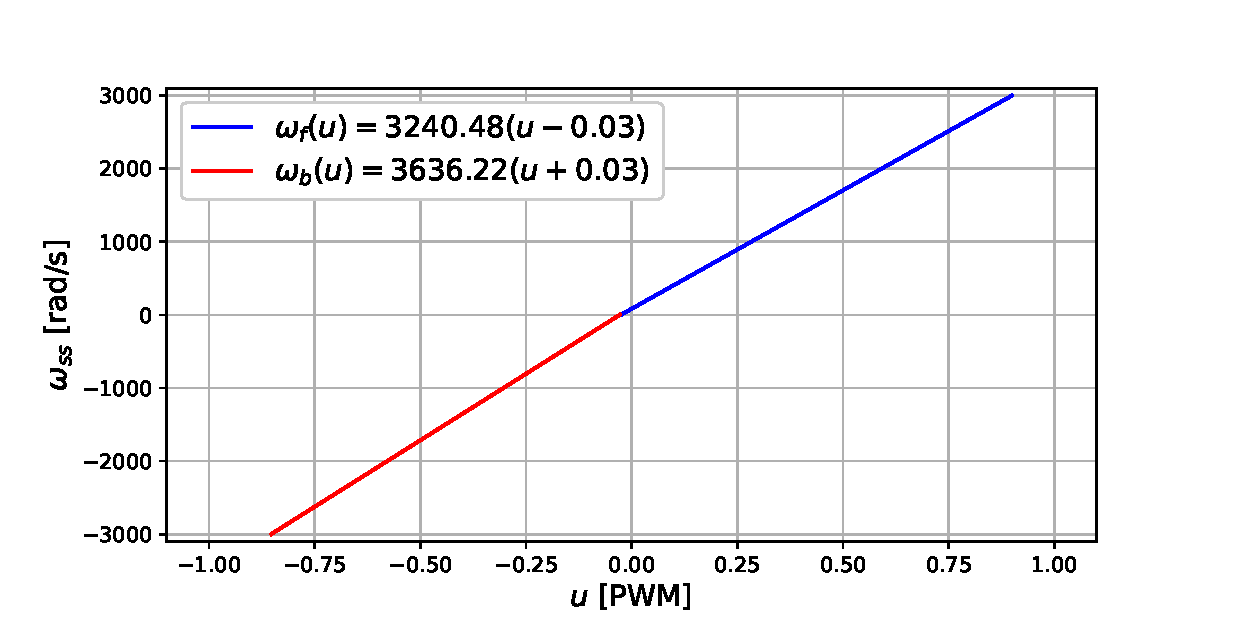
\includegraphics[width=\textwidth]{figuras/resultados/exp04/curva_feedforward_esquerdo100.eps}
        \caption{Motor esquerdo.}
    \end{subfigure}
    \begin{subfigure}{.45\textwidth}
        \centering
        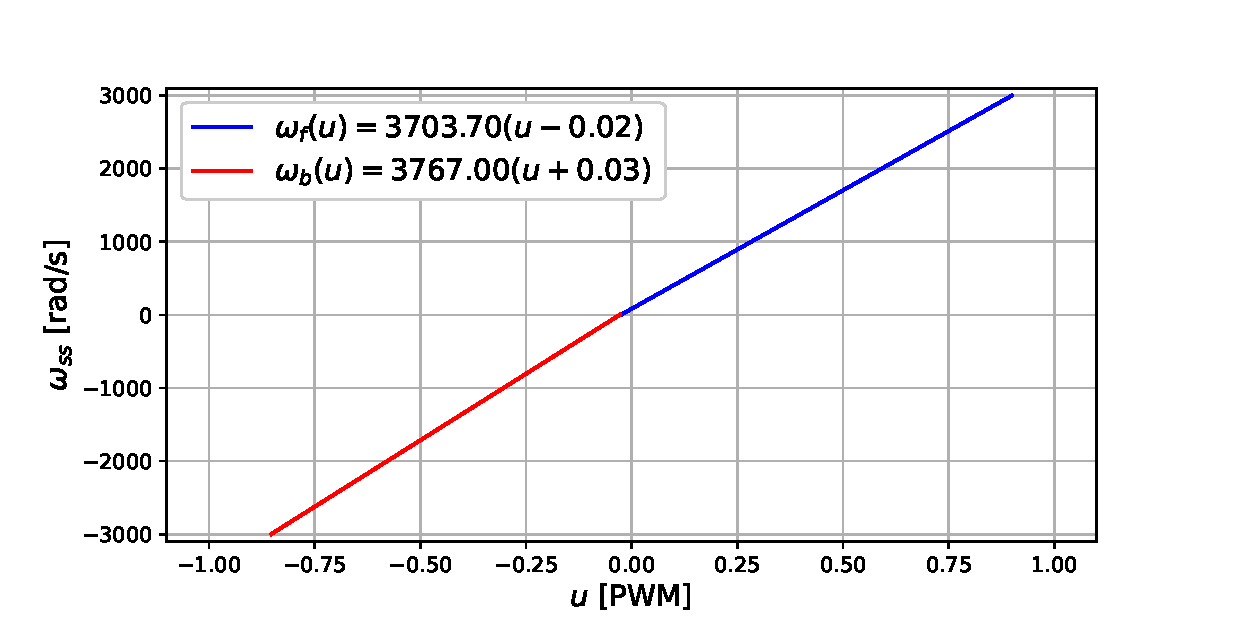
\includegraphics[width=\textwidth]{figuras/resultados/exp04/curva_feedforward_direito100.eps}
        \caption{Motor direito.}
    \end{subfigure}
    \caption{Curva $\omega_{ss}(u)$.}
\end{figure}

\end{frame}

\begin{frame}{Resultado da Aproximação do Comportamento do Sistema}


\begin{figure}
    \begin{subfigure}{.45\textwidth}
        \centering
        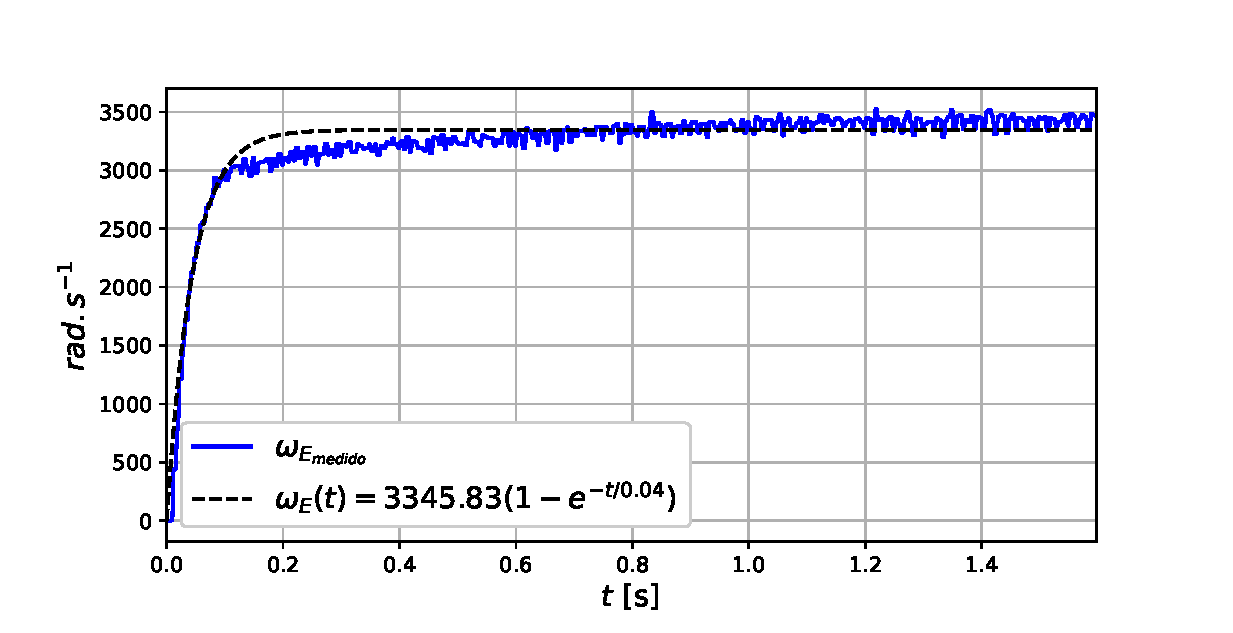
\includegraphics[width=\textwidth]{figuras/resultados/exp04/regressao_vs_medido_esquerdo100.eps}
        \caption{Motor Esquerdo.}
    \end{subfigure}
    \begin{subfigure}{.45\textwidth}
        \centering
        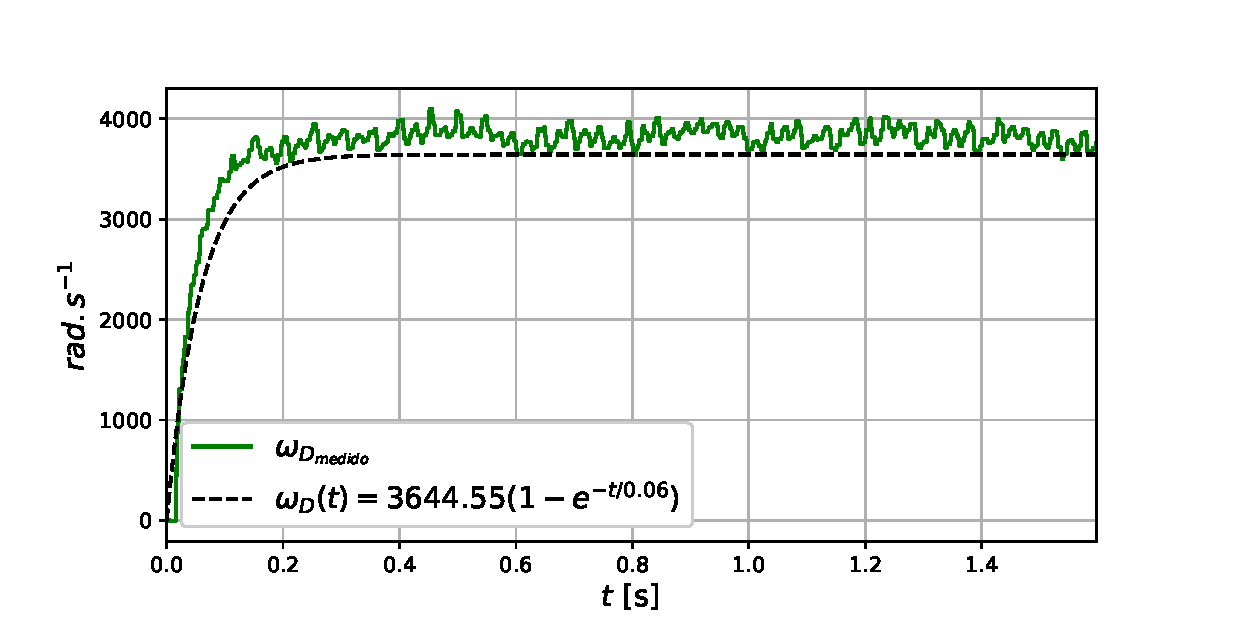
\includegraphics[width=\textwidth]{figuras/resultados/exp04/regressao_vs_medido_direito100.eps}
        \caption{Motor Direito.}
    \end{subfigure}
    \caption{Curva $\omega(t)$ teórica versus $\omega_{\text{medido}}$.}
\end{figure}
    
\end{frame}


\begin{frame}{Resultado da Filtragem}

    \begin{figure}
        \begin{subfigure}{.45\textwidth}
            \centering
            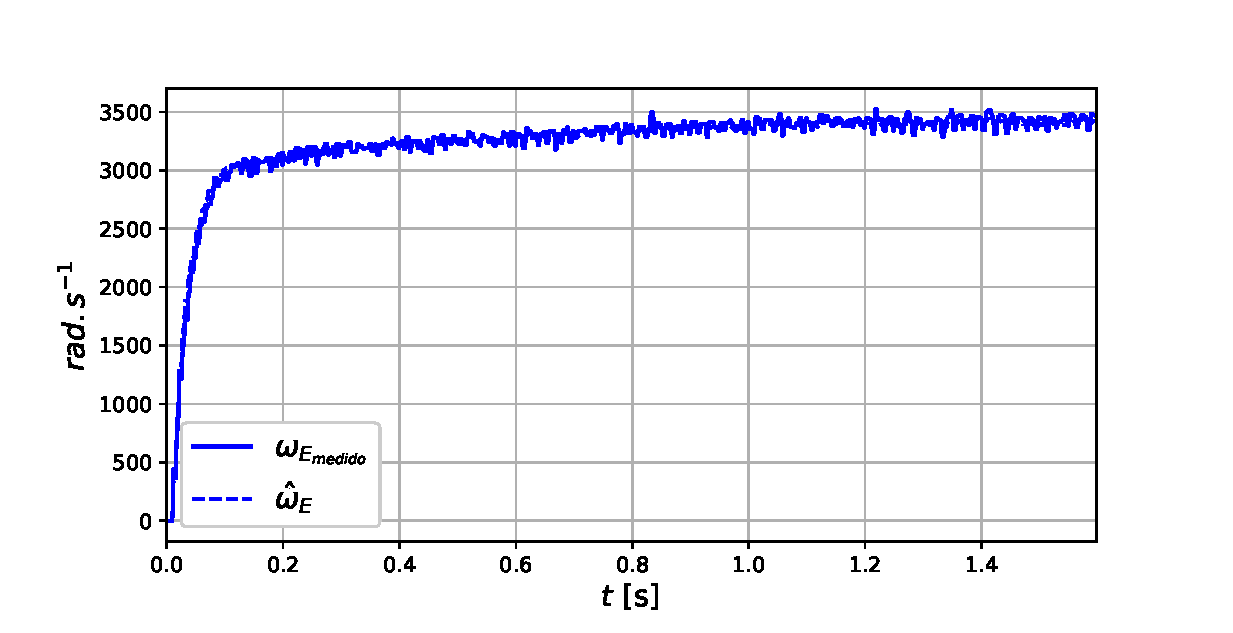
\includegraphics[width=\textwidth]{figuras/resultados/exp04/filtro_vs_sem_filtro_esquerdo100.eps}
            \caption{Motor Esquerdo.}
        \end{subfigure}
        \begin{subfigure}{.45\textwidth}
            \centering
            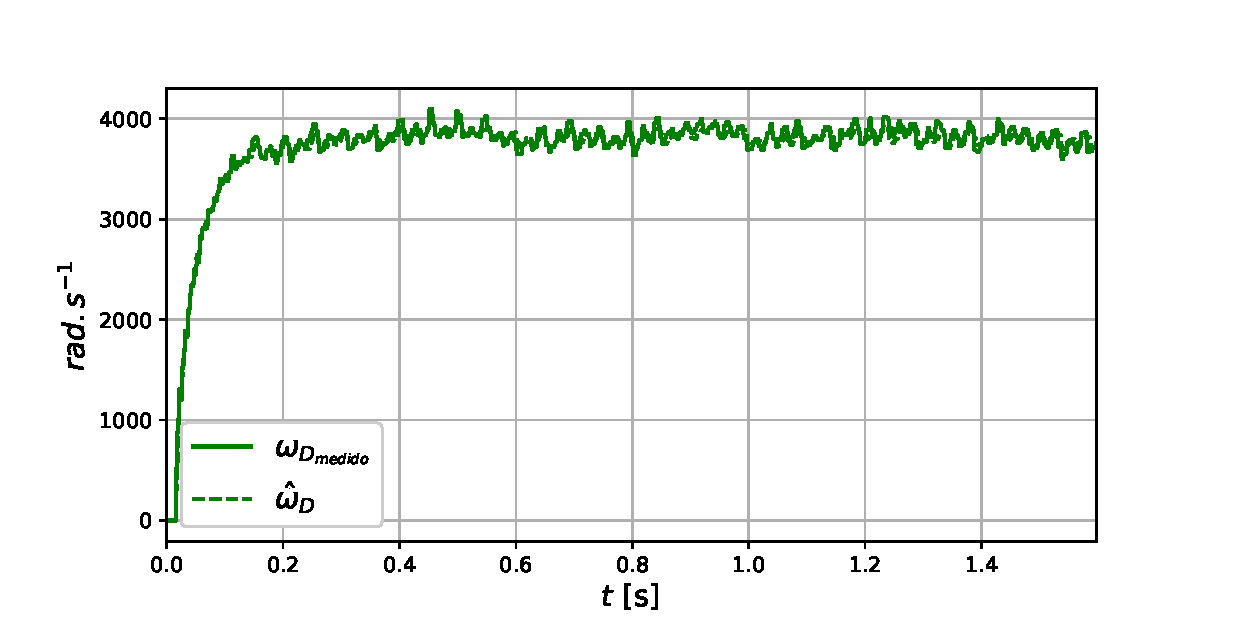
\includegraphics[width=\textwidth]{figuras/resultados/exp04/filtro_vs_sem_filtro_direito100.eps}
            \caption{Motor Direito.}
        \end{subfigure}
        \caption{Comparação entre a velocidade estimativa $\hat{\omega}$ e a velocidade $\omega$ medida.}
    \end{figure}
    
\end{frame}

\begin{frame}{Resultado do Controle}

    \begin{figure}
        \centering
        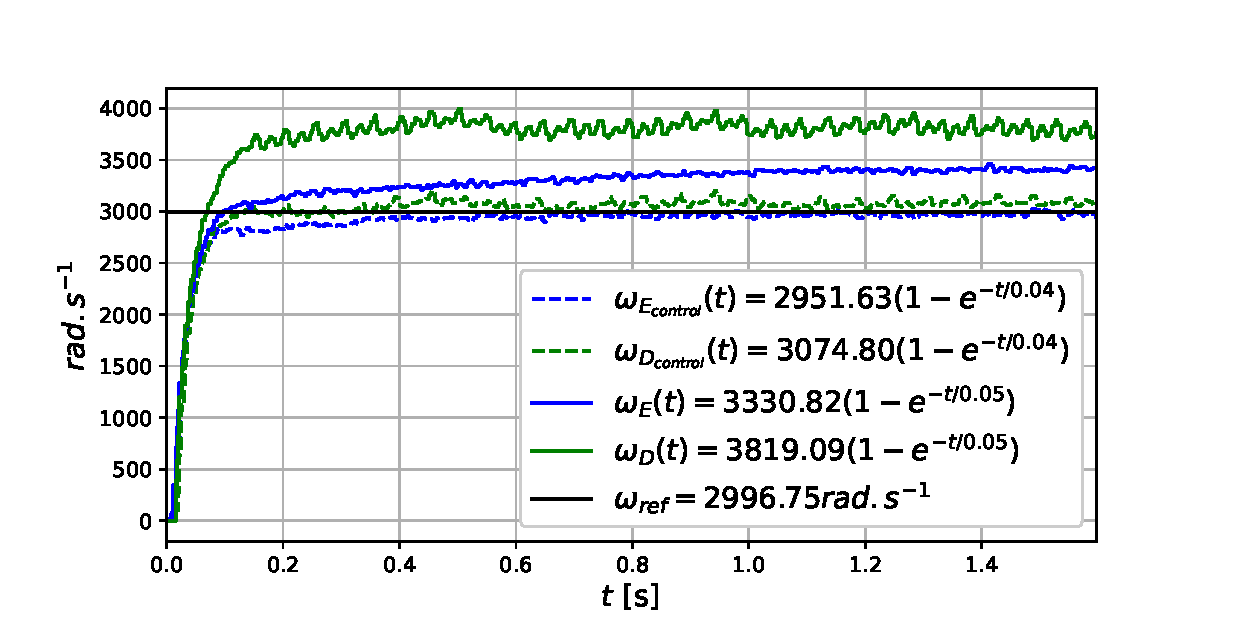
\includegraphics[width=0.6\textwidth]{figuras/resultados/exp04/controlador_vs_sem_controlador100.eps}
        \caption{Comparação entre o sistema com controlador e sem controlador.}
    \end{figure}
    
\end{frame}

\begin{frame}{Comparação}
    \begin{figure}
        \centering
        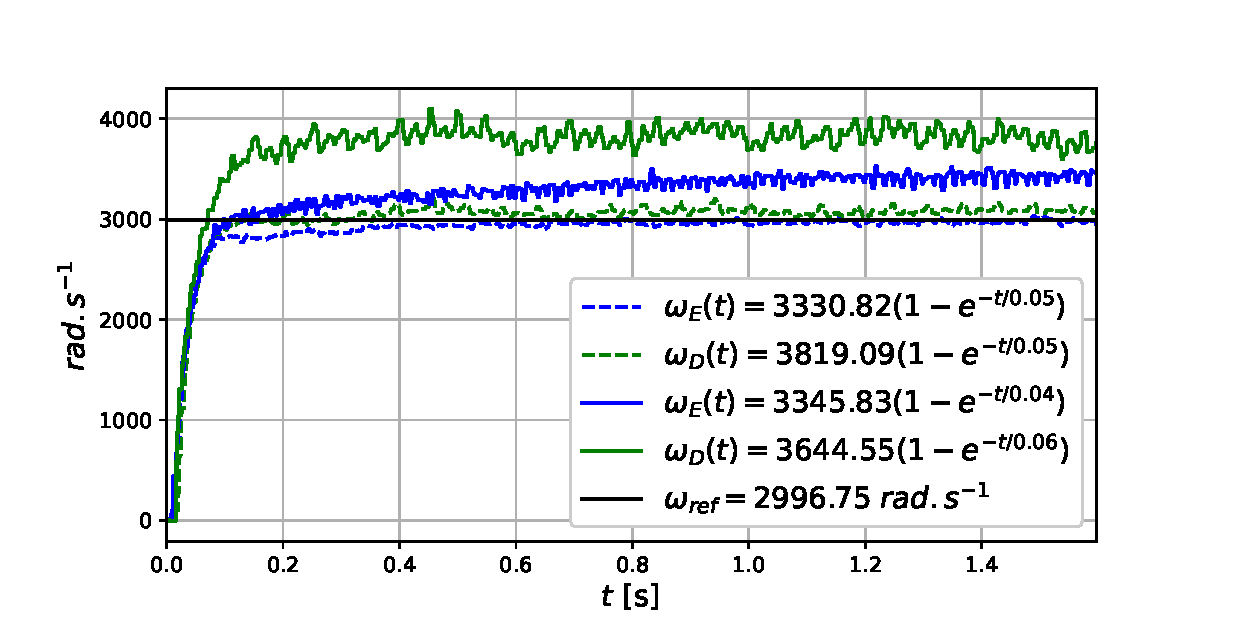
\includegraphics[width=0.6\textwidth]{figuras/resultados/exp04/antes_vs_depois100.eps}
        \caption{Resposta sem o filtro de \emph{kalman} e sem controle versus com controlador e com o filtro.}
    \end{figure}
\end{frame}





% Conclusao
\section{Conclusões e Trabalhos Futuros}
\begin{frame}{Conclusões e Trabalhos Futuros}
Conclusões:
    \begin{itemize}
        \item Comportamento da planta foi como o esperado;
        \item Filtro de \emph{Kalman} conseguiu reduzir bastante o erro de quantização;
        \item Esquema de controle com bons resultados.
    \end{itemize}

Trabalhos Futuros:    
    \begin{itemize}
        \item Adição da ação integral;
        \item Calibração automática.
    \end{itemize}
\end{frame}


% Referencias
% \section{Referencias}
\begin{frame}{Referências}
	Suas referencias bibliográficas aqui, siga o modelo ABNT.
	\bibliography{bib/bibliografia}
\end{frame}

% Agradecimentos
% \section{}
% \begin{frame}{Agradecimentos}
% 	Agradeço a todos. 	
% \end{frame}

\end{document}